\documentclass[12pt,a4paper]{report}
\usepackage[utf8]{inputenc}

\usepackage[T1]{fontenc} %to search pdf
\usepackage{ucs}
\usepackage{amsmath, amssymb}
\usepackage{amsfonts}
\usepackage{amssymb}
\usepackage[english]{babel} % Comentário, Português do Brasil
\usepackage{graphicx}
\usepackage{setspace}
\usepackage{fancyhdr}
\usepackage[pdftex, colorlinks,linkcolor=black,hyperindex]{hyperref}
\usepackage{wrapfig}
\usepackage{wallpaper}
\usepackage{subfig}
\usepackage{float}
\usepackage{esvect}


\hypersetup{
    colorlinks,
    citecolor=black,
    filecolor=black,
    linkcolor=black,
    urlcolor=blue
}

\author{Centro de Tecnologia da Informação Renato Archer}
\title{InVesalius - User guide}
\date{}

\begin{document}

\thispagestyle{empty}

\begin{flushright}

\flushright \scalebox{2.5}{\sffamily{\textbf{InVesalius}}}
\par
\vspace{180pt}
\scalebox{2.8}{\sffamily User Guide}
\ThisLLCornerWallPaper{1}{../user_guide_figures/capa2.png}

\begin{figure}[h!]
\flushright 

\includegraphics[scale=0.5, bb = 0 0 300 601]{../user_guide_figures/logo_cti.jpg}
\end{figure}		

\end{flushright}
\newpage
\vspace*{10pt}
\thispagestyle{empty}

\begin{center} \emph{\begin{large}  About InVesalius \end{large}}
\vspace{2pt}
\end{center}

\onehalfspacing
 		
InVesalius is public health software that performs analysis and segmentation of
Virtual anatomical models, enabling the creation of physical models with the aid of
rapid prototyping (3D printing).
From two-dimensional (2D) images obtained through Computed Tomography (CT) or Magnetic Resonance Imaging (MRI), the program allows users to create
three-dimensional (3D) anatomical representations of patients for further medical use.

InVesalius is named in honour of the Belgian doctor Andreas Vesalius (1514-1564), widely
considered the father of modern anatomy.
InVesalius software is developed by CTI (Center for Information Technology Center Renato
Archer), a unit of the Brazilian Ministry of Science and Technology (MCT), since 2001. Initially, only
the installation program was distributed as freeware. In November 2007
InVesalius was made fully available as free software and open source via the Public Software Portal, allowing for communities of users and developers to connect.
InVesalius is, in short, a simple yet robust, free cross-platform tool that is easy to use.


The use of visualization technologies and three-dimensional analysis of medical images, when combined with rapid prototyping (3D printing), assists the surgeon in diagnosing pathologies and a detailed surgical planning and simulation of complex process in advance, which may involve, for example, a high degree of facial deformity or integration of prosthetics.

InVesalius has demonstrated great versatility and has applications in different areas, including medicine, dentistry, veterinary medicine, archeology and engineering.

Download options:

\begin{itemize}
	\item \href{https://www.cti.gov.br/invesalius}{https://www.cti.gov.br/invesalius}
	\item \href{http://invesalius.github.io}{http://invesalius.github.io}	
	\item \href{http://www.softwarepublico.gov.br}{www.softwarepublico.gov.br}
\end{itemize}
		
\noindent
\tableofcontents
\chapter{Introduction}

This manual aims to guide end users in the application of InVesalius tools and also presents some concepts to facilitate the use of the software.

InVesalius is software that is designed to assist health professionals on diagnosis and surgical planning. It should be noted, however, that all software in the diagnostic context is fully supplementary, and each and every act committed is the responsibility of health professionals.
 
In addition to medicine, InVesalius can be utilized in other areas such as archeology, medicine, dentistry, veterinary, or even in industrial applications. As a basic requirement, the images to be analyzed are in DICOM (Digital Imaging Communications in Medicine). To date, InVesalius reconstructs images stemmed from CT scanners and MRI machines. To operate the software, basic computer literacy is essential. Understanding medical images can help to form a better understanding of the operations.

\section{Important Concepts}

Detailed in this section are a list of concepts essential to better understand and operate the software.

\subsection{DICOM (\textit{Digital Image Communications in Medicine})}	

DICOM is a standard the transmission, storage and treatment of medical images. The standard encompasses various origins of medical images, such as images emanating from computed tomography (CT) equipment, magnetic resonance, ultrasound, and electrocardiogram, among others.

A DICOM image consists of two main components, namely, an array containing the pixels of the image and a set of meta-information. This information includes, but is not limited to, patient name, mode image and the image position in relation to the space (in the case of CT and MRI).

\subsection{Computed Tomography - Medical}

Computed tomography indicates the radiodensity of tissues, i.e., the average X-ray absorption by the tissues. The radiodensity reading is translated into an image gray levels, called the Hounsfield scale, named Godfrey Newbold Hounsfield, one of the creators of the first CT scan.

\begin{figure}[!htb]
\centering
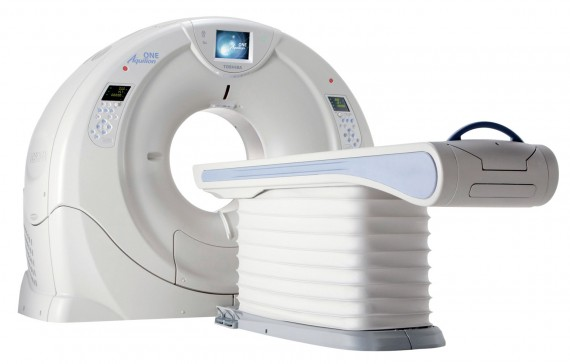
\includegraphics[scale=0.4]{../user_guide_figures/tomografo.jpg}
\caption{Medical CT scanner - www.toshibamedical.com.br}
\end{figure}

Most modern CT scanning appliances are equipped with a radiation emitter and a sensor bank (with channels ranging from 2 to 256), which circle the patient while the stretcher is moved, forming a spiral. This generates a large number of images simultaneously, with little emission of X-rays.

\subsubsection{Hounsfield Scale}

As mentioned in the previous section, the CT images are generated in gray levels, expressed in Hounsfield (HU), wherein lighter shades represent denser matters, and the darker, less dense matter such as skin and brain tissues. 

Table~\ref{tab:escala_hounsfield} presents some materials and their respective values in Hounsfield Units (HU).

\begin{table}[h]
\centering
\caption{Escala de Hounsfield}
\begin{tabular}{lcc}\\
\hline % este comando coloca uma linha na tabela
Material & HU\\
\hline
\hline
Air & -1000 or less\\
Fat & -120\\
Water & 0\\
Muscle & 40\\
Contrast & 130\\
Bone & 400 or more\\
\hline
\end{tabular}
\label{tab:escala_hounsfield}
\end{table}


\subsection{Computed Tomography - Dental (CBCT)}

The dental CT commonly works with less radiation emission compared to medical CT, and therefore makes it possible to view more details of delicate regions such as alveolar cortical.

\begin{figure}[!htb]
\centering
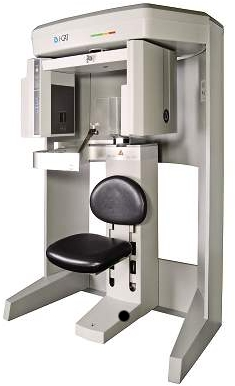
\includegraphics[scale=0.4]{../user_guide_figures/feixe_conico.jpg}
\caption{Dental tomography - www.kavo.com.br}
\end{figure}

Image acquisition is performed with the patient positioned vertically (as opposed to medical tomography in which the patient is horizontal). A transmitter X-ray surround the patient's skull, forming an arc of $180^\circ$ or $360^\circ$. The images generated are compiled as a volume of the patient's skull. This volume is then "sliced" by the software into individual layers, being able to generate images with different spacing or fields of view, such as a panoramic view of the region of interest.

The images acquired by dental scanners often require more post processing when it is necessary to separate (segmental) certain structures using other software such as InVesalius. This is because, typically, these images have more gray levels than, which makes use of segmentation patterns (preset) less. Another very common feature in the images of provincial dental CT scanners is the high presence of speckle noise and other forms of noise typically caused by the presence of amalgam prosthetics.

\subsection{Magnetic Resonance Imaging - MRI}

MRI is an examination performed without the use of ionizing radiation. Instead, it use a strong magnetic field to align the atoms of any element present in our body, most commonly hydrogen. After alignment, radio waves are triggered to excite atoms. The sensors measure the time that the hydrogen atoms take to realign. This makes it possible to distinguish between different tissues, as different types possess different quantities of hydrogen atoms.

To avoid interference and improve the quality of the radiofrequency signal, the patient is placed inside a narrow tube encompassed by the coil and scanning unit.

\begin{figure}[!htb]
\centering
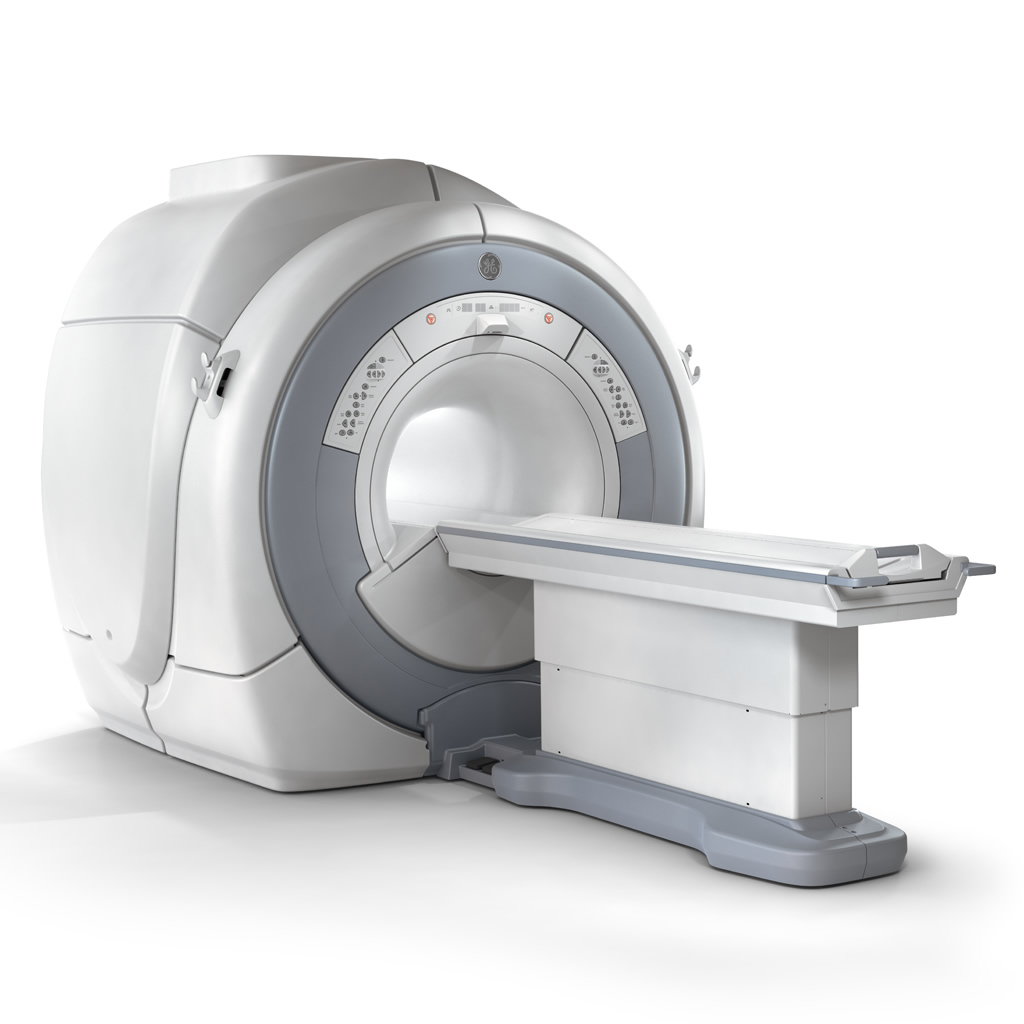
\includegraphics[scale=0.2]{../user_guide_figures/rm_ge.jpg}
\caption{Magnetic resonance imaging equipment - www.gehealthcare.com}
\end{figure}

\begin{figure}[!htb]
\centering
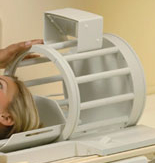
\includegraphics[scale=0.8]{../user_guide_figures/bobina.jpg}
\caption{Coil - www.healthcare.philips.com}
\end{figure}

\subsection{Neuronavigation}
\label{sec:neuronavegador_intro}

Neuronavigation is a technique that allows tracking and localization of surgical instruments relative to neuronal
structures through computer visualization. In addition, neuronavigation systems a fundamental tool to aid surgical plan and to increase the accuracy of experiments in neuroscience, such as transcranial magnetic stimulation (TMS), electroencephalography (EEG), magnetoencephalography (MEG) and near-infrared spectroscopy (NIRS).
Despite the vast field of applications, the use of neuronavigation in research centers is limited by its high cost.
InVesalius Navigator offers users a low-cost, open-source alternative to commercial neuronavigation systems. In this sense, it is possible to use specific tools for
neuronavigation and still have the possibility of developing features on demand. The software for neuronavigation is distributed in an executable version compatible with Windows 7, 8 and 10 operating system. The chapter~\ref{sec:neuronavegador} goes into details of all features of neuronavigation in InVesalius.

\section{Resources needed}

InVesalius is designed to run on personal computers, such as desktops and notebooks. Currently, it is compatible with the following operating systems:

\begin{itemize}
	\item Microsoft Windows (Windows 7, 8, 10)
	\item GNU/Linux (Ubuntu, Mandriva, Fedora) 
	\item Apple Mac OS X
\end{itemize}

The performance of InVesalius depends mainly on the amount of reconstructed slices (images offered by the software), the amount of random access memory (RAM) available, the processor clock rate \& frequency, and operating system architecture (32-bit or 64-bit).

It is important to note that, as a general rule, the greater the amount of RAM available on the system, the greater the number of slices that can be opened simultaneously. For example, with 1 GB of available memory, it can open about 300 slices with a resolution of 512x512 pixels. With 4 GB of memory, around 1000 images can be opened simultaneously at the same resolution.

\subsection{Minimum settings}

\begin{itemize}
	\item 32-bit Operating System
	\item Intel Pentium 4 or equivalent 1.5 GHz
	\item 1 GB of RAM
	\item 10 GB available hard disk space
	\item Graphics card with 64 MB memory
	\item Video resolution of 1024x768 pixels
\end{itemize}


\subsection{Recommended settings}
\begin{itemize}
	\item 64-bit Operating System
	\item Intel Core 2 Duo processor or equivalent 2.5 GHz
	\item 8 GB of RAM
	\item 20 GB available hard disk space
	\item NVidia or ATI graphics card with 128 MB of memory
	\item Video resolution of 1920x1080 pixels
\end{itemize}



\chapter{Installation}

\section{MS-Windows}


To install InVesalius on MS-Windows, simply run the installer program. When a window asking you to confirm the file execution appears, click \textbf{Yes}.

\begin{figure}[!htb]
\centering
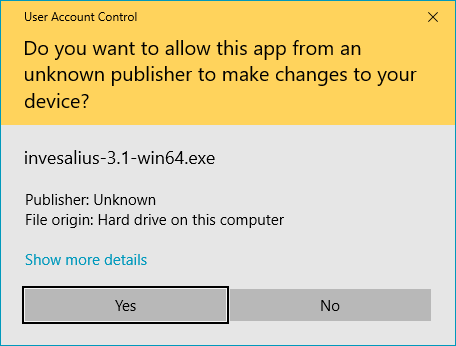
\includegraphics[scale=0.5]{installation_exec_en.png}
\end{figure}

\newpage

A new window will ask you to select the language of the installer. Select the language and click \textbf{OK}.

\begin{figure}[!htb]
\centering
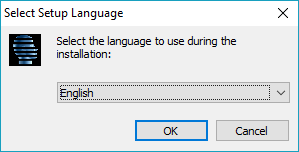
\includegraphics[scale=0.7]{installation_select_language_en.png}
\end{figure}
 
\hspace{.2cm}

The Setup installer will appear. Click \textbf{Next}.

\begin{figure}[!htb]
\centering
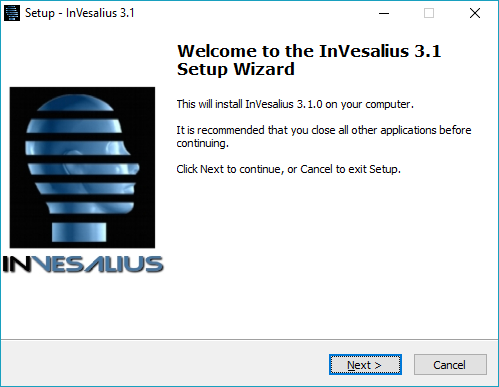
\includegraphics[scale=0.7]{installation_welcome_en.png}
\end{figure}

\newpage

Select \textbf{I accept the agreement} and click on \textbf{Next} button.

\begin{figure}[!htb] 
\centering
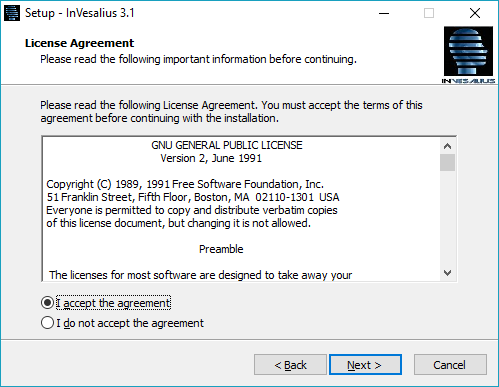
\includegraphics[scale=0.7]{installation_license_en.png}
\end{figure}

\hspace{.2cm}

Select the preferred destination for the InVesalius program files, then click \textbf{Next}.

\begin{figure}[!htb]  
\centering
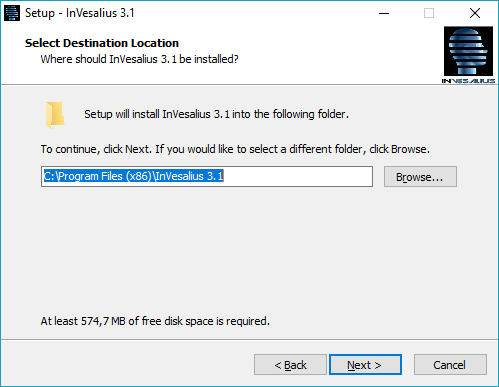
\includegraphics[scale=0.7]{installation_folder_en.png}
\end{figure}

\newpage

Click on \textbf{Next}  button.
\begin{figure}[!htb]
\centering
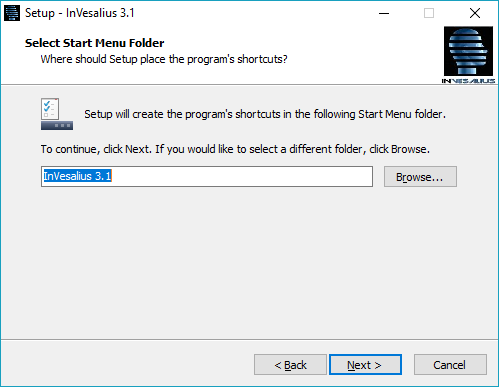
\includegraphics[scale=0.7]{installation_program_name_en.png}
\end{figure}

\hspace{.2cm}

Select \textbf{Create a desktop shortchut} and click on \textbf{Next}.

\begin{figure}[!htb]
\centering
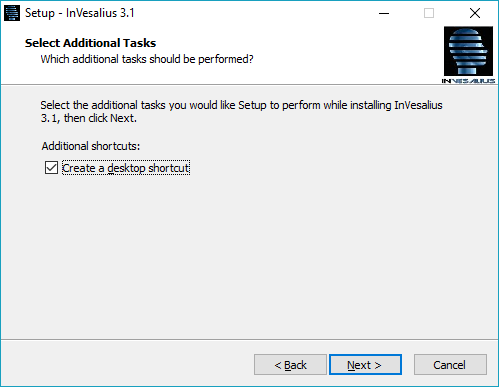
\includegraphics[scale=0.7]{installation_desktop_shortcut_en.png}
\end{figure}

\newpage

Click on \textbf{Install} button.

\begin{figure}[!htb]
\centering
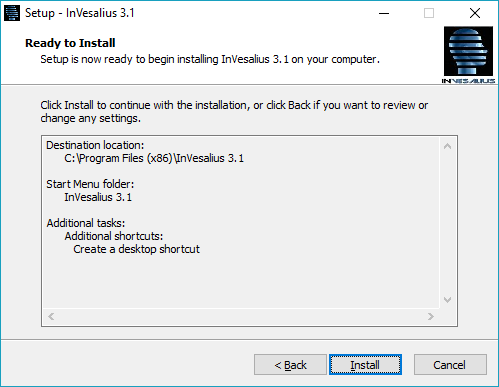
\includegraphics[scale=0.7]{installation_resume_en.png}
\end{figure}

\hspace{.2cm}

While the software is being installed, a progress window will appear.

\begin{figure}[!htb]
\centering
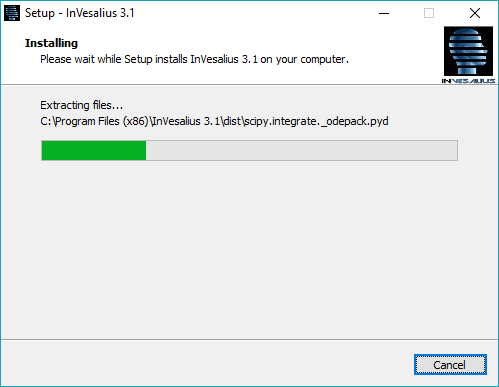
\includegraphics[scale=0.7]{installation_progress_en.png}
\end{figure}

\newpage

To run InVesalius after installation, check \textbf{Lauch InVesalius 3.1} and click on \textbf{Finish} button.

\begin{figure}[!htb]
\centering
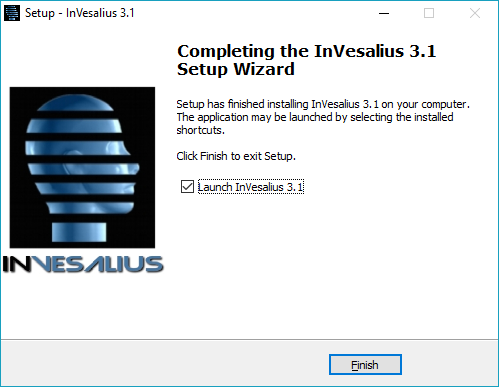
\includegraphics[scale=0.7]{installation_finish_en.png}
\end{figure}

\hspace{.2cm}

When being run for the first time, a window will appear to select the InVesalius language. Select the desired language and click \textbf{OK}.

\begin{figure}[!htb]
\centering
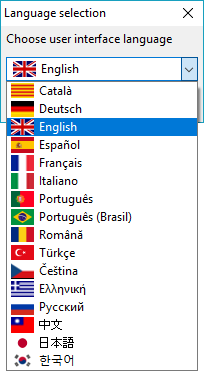
\includegraphics[scale=0.6]{invesalius_language_select_en.png}
\end{figure}

\newpage

While InVesalius is loading, the opening window shown below will be displayed.

\begin{figure}[!htb]
\centering
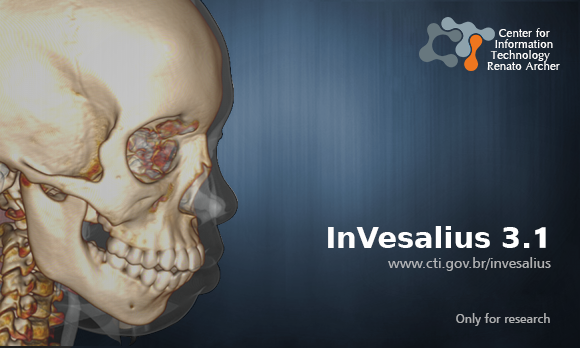
\includegraphics[scale=0.4]{splash_en.png}
\end{figure}

\hspace{.2cm}

The main program window will then open, as shown below.

\begin{figure}[!htb]
\centering
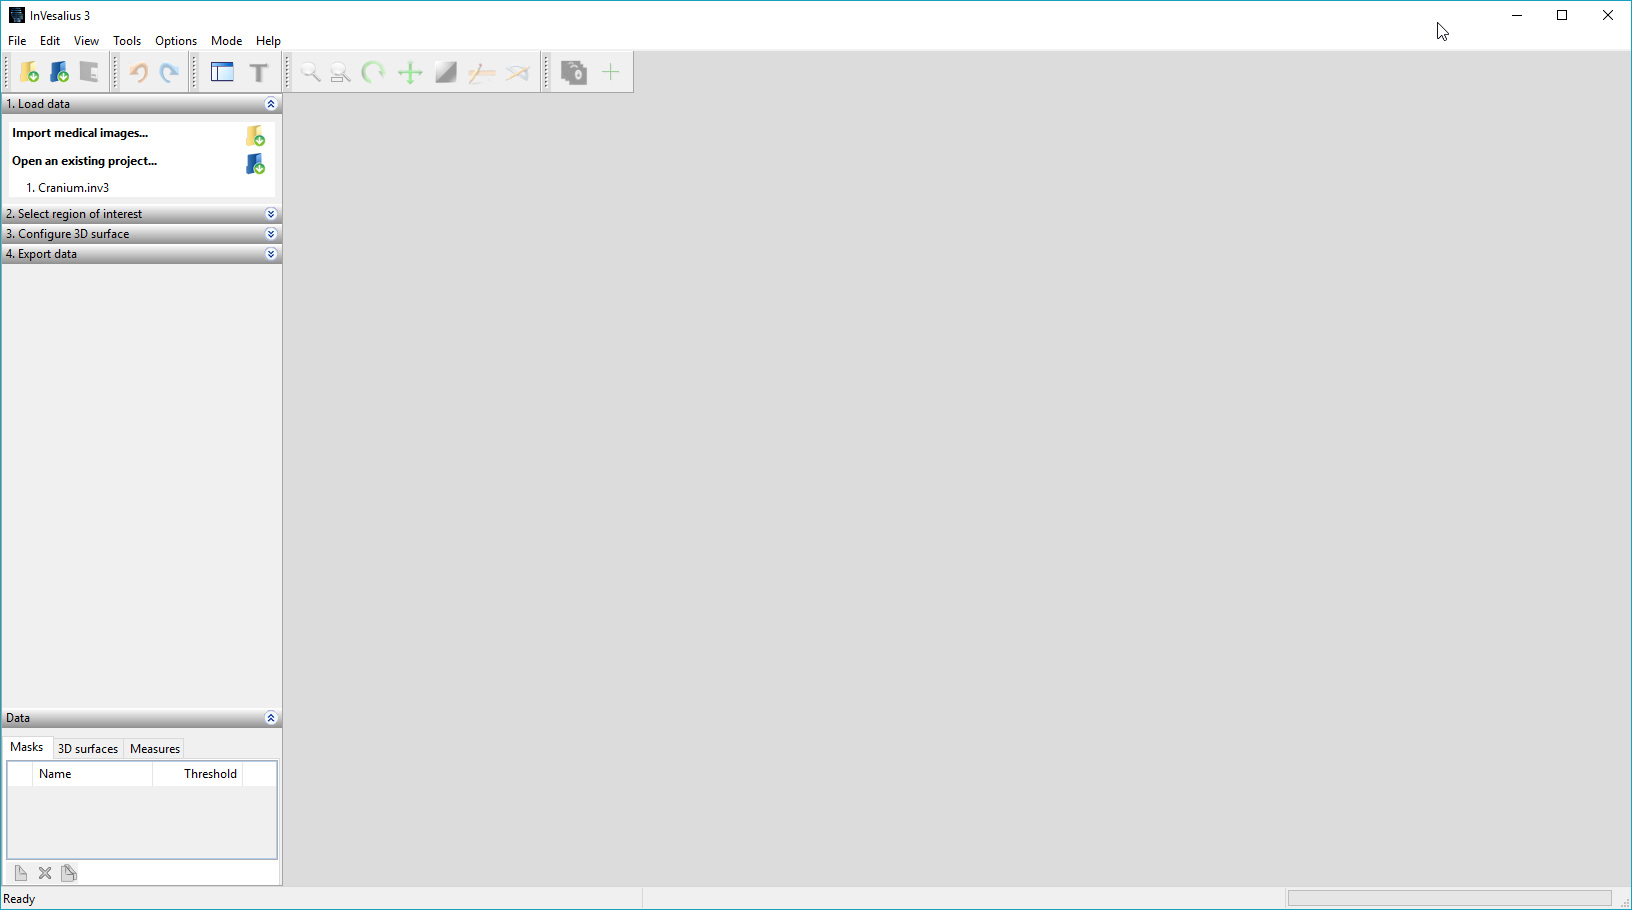
\includegraphics[scale=0.3]{main_window_without_project_en.png}
\end{figure}

\section{Mac Os X}

To start the installation on Mac OS X, double-click the installer with the left mouse button to begin installation.

\begin{figure}[!htb]
\centering
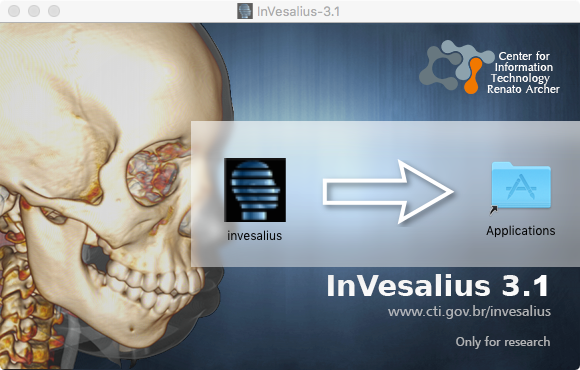
\includegraphics[scale=0.3]{mac2.png}
\end{figure}

Hold down the left button on the InVesalius software icon and drag it to the Applications folder. Both are contained in the installer.

\begin{figure}[!htb]
\centering
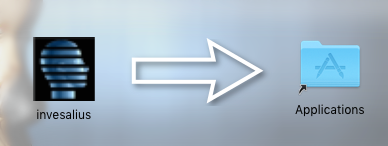
\includegraphics[scale=0.4]{mac4.png}
\end{figure}

The software is already installed, just access through the menu.
\chapter{Image import}

InVesalius imports files in DICOM format, including compressed files (lossless JPEG), Analyze (Mayo Clinic$^\copyright$), NIfTI, PAR/REC, BMP, TIFF, JPEG and PNG formats.

\section{DICOM}

Under the File menu, click on Import DICOM or use the shortcut Ctrl+I. Additionally, DICOM files can be imported by clicking on the icon shown in Figure~\ref{fig:import}.

\begin{figure}[!htb]
\centering

\includegraphics[scale=0.2]{../user_guide_figures/icons/file_import_original.png}
\caption{Shortcut to DICOM import}
\label{fig:import}
\end{figure}

\hspace{.2cm}

Select the directory containing the DICOM files, as in Figure~\ref{fig:win_folder}. InVesalius will search for files also in subdirectories of the chosen directory,
if they exist.

\newpage

Once the directory is selected, click \textbf{OK}.

\begin{figure}[!htb]
\centering
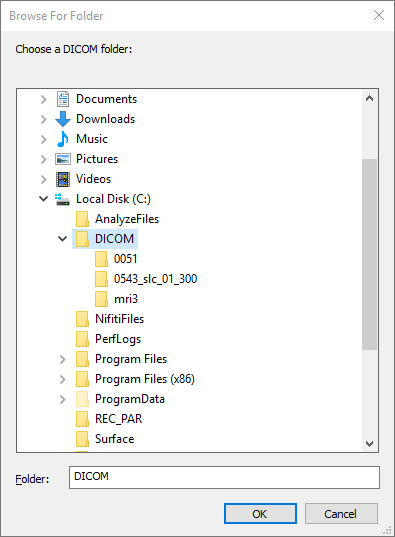
\includegraphics[scale=0.5]{../user_guide_figures/invesalius_screen/import_select_folder_en.png}
\caption{Folder Selection}
\label{fig:win_folder}
\end{figure}

\hspace{.2cm}

While InVesalius search for DICOM files in the directory, the loading progress of the scanned files is displayed, as shown in the Figure~\ref{fig:ver_file}.

\begin{figure}[!htb]
\centering
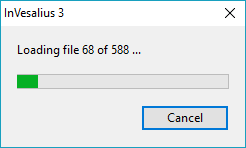
\includegraphics[scale=0.6]{../user_guide_figures/invesalius_screen/import_load_files_en.png}
\caption{Loading file status}
\label{fig:ver_file}
\end{figure}

\newpage

If DICOM files are found, a window open (shown Figure~\ref{fig:win_import}) will open to select the patient and respective series to be opened. It is also possible to skip images for reconstruction.

\begin{figure}[!htb]
\centering
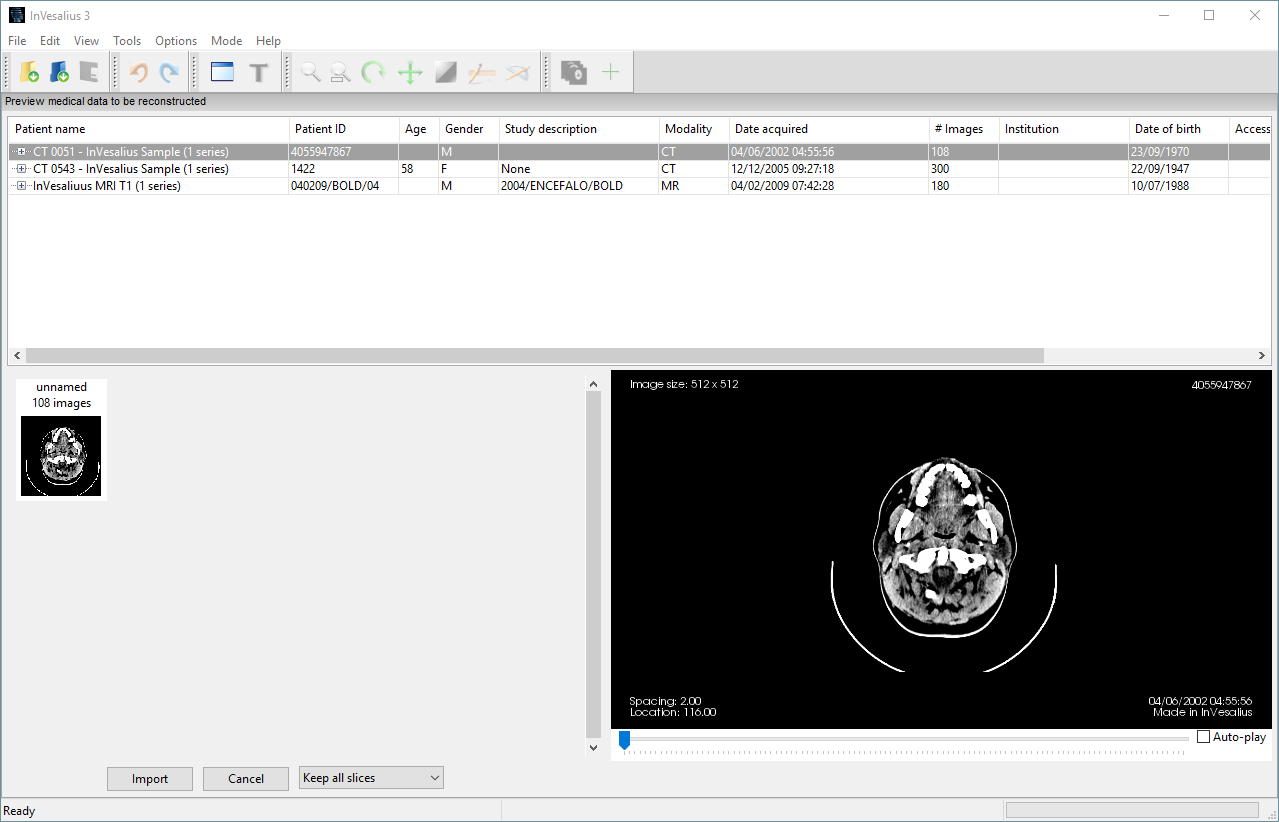
\includegraphics[scale=0.4]{../user_guide_figures/invesalius_screen/import_window_en.png}
\caption{Import window}
\label{fig:win_import}
\end{figure}

\newpage

To import a series with all images present, click "\textbf{$+$}" on the patient’s name to expand the corresponding series. Double-click on the description of the series. See Figure~\ref{fig:import_serie}.

\begin{figure}[!htb]
\centering
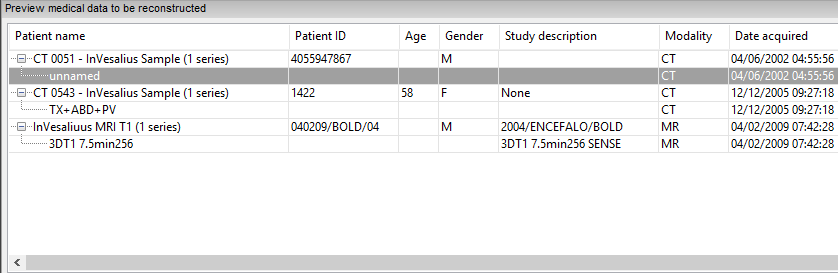
\includegraphics[scale=0.5]{../user_guide_figures/invesalius_screen/import_window_detail_en.png}
\caption{Series selection}
\label{fig:import_serie}
\end{figure}

In some cases, when there is no computer with memory and/or satisfactory processing to work with large numbers of images in a series, it is recommended to skip some of them. To do this, click \textbf{once} with the \textbf{left} mouse button over the description of the series (Figure~\ref{fig:import_serie}) and select how many images will be skipped (Figure~\ref{fig:skip_image}), then click \textbf{Import}.

\begin{figure}[!htb]
\centering
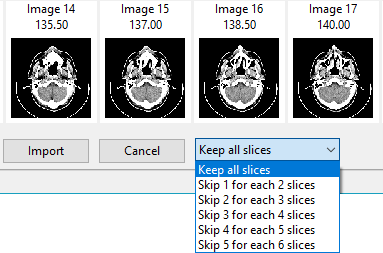
\includegraphics[scale=0.6]{../user_guide_figures/invesalius_screen/import_window_skip_slice_en.png}
\caption{Skip imagens option}
\label{fig:skip_image}
\end{figure}

If there is an insufficient amount of available memory at the time of loading the images it is recommended that the resolution of the slices be reduced to work with volumetric and surface visualization, as shown in Figure~\ref{fig:resize_image}.
The slices will be resized according to the percentage relative to the original resolution. For example, if each slice of the exam the dimension of 512 x 512 pixels and the "Percentage of original resolution" is suggested to be 60 \%, each resulting image will be 307 x 307 pixels. To open with the original pixel resolution, set the percentage to 100.

\begin{figure}[!htb]
\centering
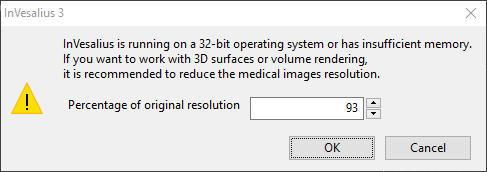
\includegraphics[scale=0.5]{../user_guide_figures/invesalius_screen/import_window_lower_memory_en.png}
\caption{Image size reduction}
\label{fig:resize_image}
\end{figure}

If the image was obtained with the gantry tilted it will be necessary to correct to avoid distortion of any reconstruction. InVesalius allows the user to do this easily. When importing an image with the gantry tilted a dialog will appear, showing the gantry tilt angle. (Figure~\ref{fig:gantry_tilt}). It is possible to change this value, but it is not recommended. Click on the \textbf{Ok} to do the correction. If you click on the \textbf{cancel} button the correction will not be done.

\begin{figure}[!htb]
\centering
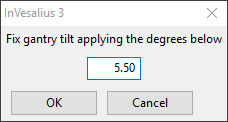
\includegraphics[scale=0.75]{../user_guide_figures/invesalius_screen/window_gantry_tilt_en.png}
\caption{Gantry tilt correction}
\label{fig:gantry_tilt}
\end{figure}

After the above procedure, a window will be displayed (Figure \ref{fig:prog_recons}) with reconstruction (when images are stacked and interpolated).

\begin{figure}[!htb]
\centering
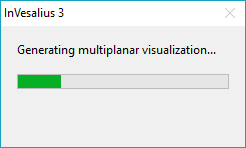
\includegraphics[scale=0.6]{../user_guide_figures/invesalius_screen/import_window_progress_en.png} 
\caption{Reconstruction progress}
\label{fig:prog_recons}
\end{figure}

\newpage

\section{Analyze}

To import Analyze files, under the \textbf{File} menu, click \textbf{Import other files}, then click in the \textbf{Analyze} option as show the Figure~\ref{fig:analyze_menu}.

\begin{figure}[!htb]
\centering
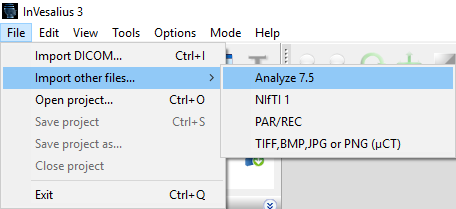
\includegraphics[scale=0.4]{../user_guide_figures/invesalius_screen/import_analyze_menu_en.png}
\caption{Menu for importing images in analyze format.}
\label{fig:analyze_menu}
\end{figure}

Select the Analyze file format (\textbf{.hdr}) and click on \textbf{Open} (Figure~\ref{fig:analyze_import}).
 
\begin{figure}[!htb]
\centering
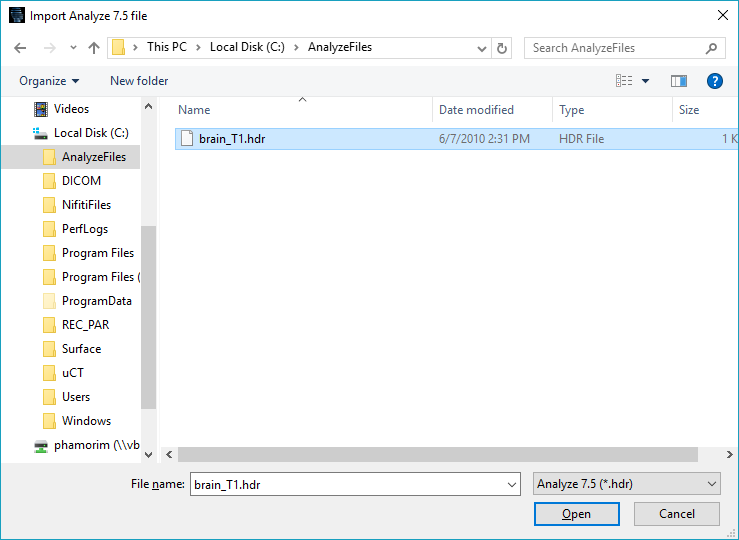
\includegraphics[scale=0.4]{../user_guide_figures/invesalius_screen/import_analyze_window_en.png}
\caption{Import analyze file format}
\label{fig:analyze_import}
\end{figure}

\section{NIfTI}

To import NIfTI files, under the \textbf{File}  menu, click \textbf{Import other files} and then click \textbf{NIfTI} as shown in Figure~\ref{fig:import_nifti_menu_pt}.


\begin{figure}[!htb]
\centering
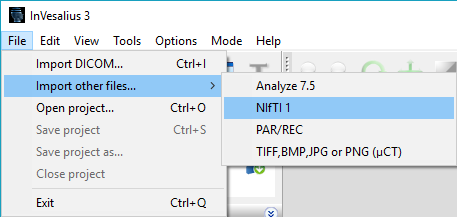
\includegraphics[scale=0.4]{../user_guide_figures/invesalius_screen/import_nifti_menu_en.png}
\caption{Menu to import images in NIfTI format}
\label{fig:import_nifti_menu_pt}
\end{figure}

Select the NIfTI file format, (either \textbf{nii.gz} or \textbf{.nii}) then click \textbf{Open} (Figure~\ref{fig:import_nifti_window_pt}). If the file is in another format as \textbf{.hdr}, select \textbf{all files(*.*)} option.

\begin{figure}[!htb]
\centering
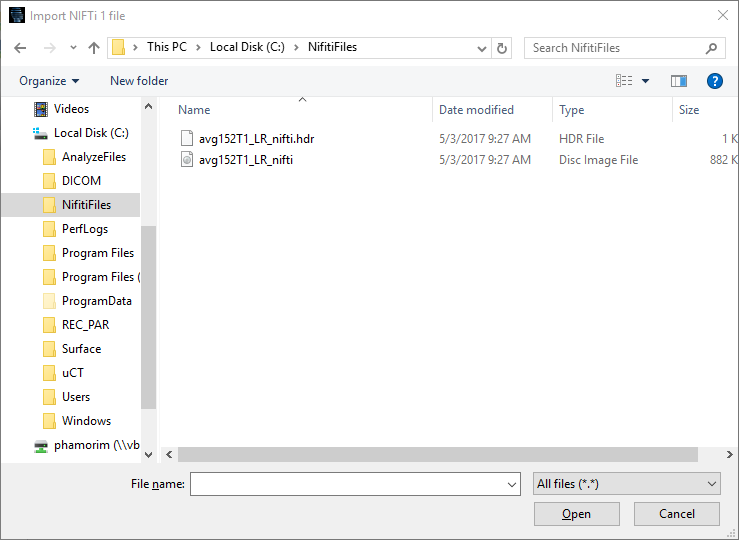
\includegraphics[scale=0.4]{../user_guide_figures/invesalius_screen/import_nifti_window_en.png}
\caption{Importing images in NIfTI format.}
\label{fig:import_nifti_window_pt}
\end{figure}

\section{PAR/REC}

To import PAR/REC file, under the \textbf{File} menu, click \textbf{Import other files}, and then click on \textbf{PAR/REC} as shown in Figure~\ref{fig:import_parrec_menu_pt}.

\begin{figure}[!htb]
\centering
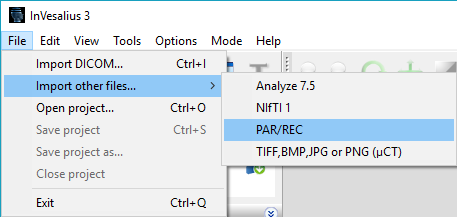
\includegraphics[scale=0.4]{../user_guide_figures/invesalius_screen/import_parrec_menu_en.png}
\caption{Menu for importing PAR/REC images}
\label{fig:import_parrec_menu_pt}
\end{figure}

Select PAR/REC file type, with the file extension \textbf{.par} and click \textbf{Open} (Figure~\ref{fig:import_parrec_window_pt}). If the file has no extension, select \textbf{all files(*.*)} option.

\begin{figure}[!htb]
\centering
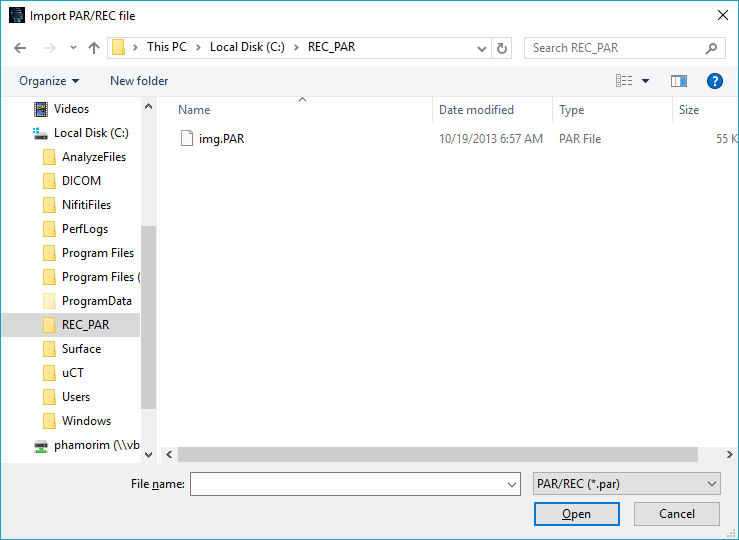
\includegraphics[scale=0.4]{../user_guide_figures/invesalius_screen/import_parrec_window_en.png}
\caption{PAR/REC import}
\label{fig:import_parrec_window_pt}
\end{figure}

\section{TIFF, JPG, BMP, JPEG or PNG (micro-CT)}

TIFF, JPG, BMP, JPEG or PNG file format for microtomography equipment (micro-CT or $\mu$CT) or others. InVesalius imports files in these formats if pixels present are represented in \textbf{grayscale}.

To import, click on menu \textbf{File}, \textbf{Import other files...} and then click on \textbf{TIFF, JPG, BMP, JPEG ou PNG ($\mu$CT)} option as shown the figure~\ref{fig:import_bmp_menu_pt}.

\begin{figure}[!htb]
\centering
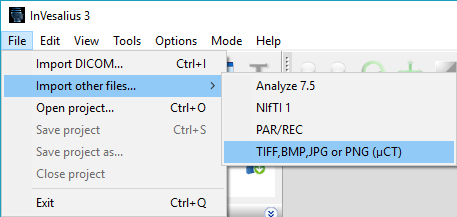
\includegraphics[scale=0.4]{../user_guide_figures/invesalius_screen/import_bmp_menu_en.png}
\caption{Import images in BMP and others formats}
\label{fig:import_bmp_menu_pt}
\end{figure}

Select the directory that contains the files, as shown the Figure~\ref{fig:import_bmp_select_folder}. InVesalius will search for files also in subdirectories of the chosen directory, if they exist. 

Click on \textbf{OK}.

\begin{figure}[!htb]
\centering
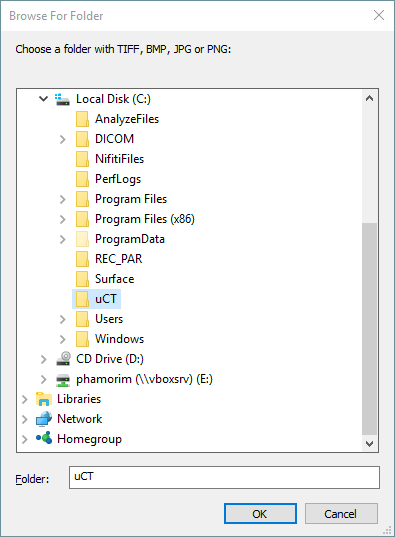
\includegraphics[scale=0.5]{../user_guide_figures/invesalius_screen/import_bmp_select_folder_en.png}
\caption{Folder selection}
\label{fig:import_bmp_select_folder}
\end{figure}

While InVesalius is looking for TIFF, JPG, BMP, JPEG, or PNG files in the directory, the upload progress of the scanned files is displayed, as illustrated in Figure~\ref{fig:import_bmp_load_pt}.

\begin{figure}[!htb]
\centering
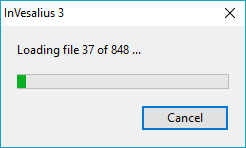
\includegraphics[scale=0.6]{../user_guide_figures/invesalius_screen/import_bmp_load_en.png}
\caption{Checking and loading files status.}
\label{fig:import_bmp_load_pt}
\end{figure}

If files in the desired formats are located, a window will open (shown in Figure~\ref{fig:import_bmp_window_pt}) to display the files eligible for reconstruction. Images can also be skipped to remove files from the rebuild list. The files are sorted according to file names. It is recommended that the files are numbered according to the desired rebuild order.

\begin{figure}[!htb]
\centering
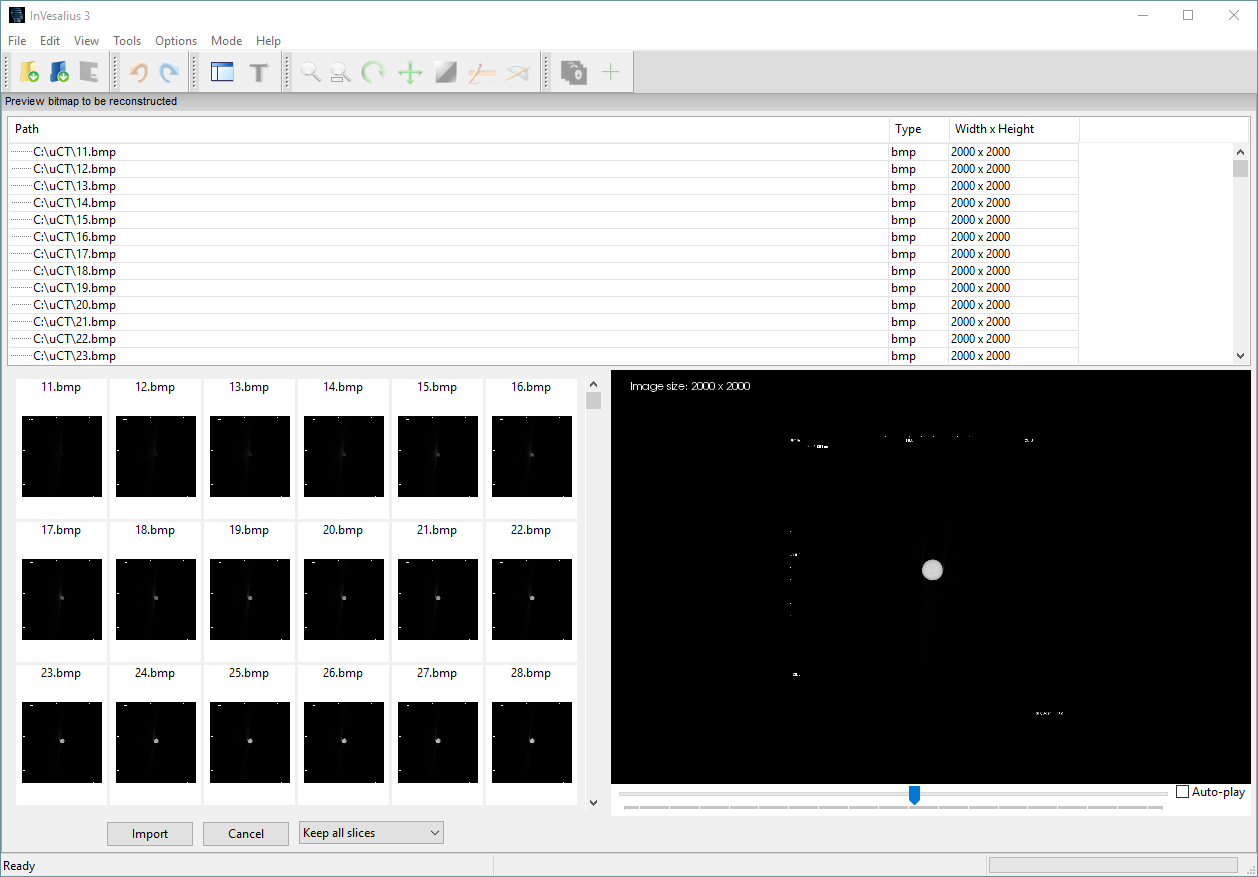
\includegraphics[scale=0.3]{../user_guide_figures/invesalius_screen/import_bmp_window_en.png}
\caption{Window to import BMP files.}
\label{fig:import_bmp_window_pt}
\end{figure}
 
To delete files that are not of interest, select a file by clicking the left mouse button and then pressing the delete key. You can also choose a
range of files to delete by clicking the \textbf{left mouse button} on a file, holding down the \textbf{shift} key, clicking again with the mouse button in the last file of the track and finally pressing the \textbf{delete} button.

Similar to when importing DICOM files, you can skip BMP images for re-building. In some cases, particularly where a computer with satisfactory memory and/or processing is unavailable, it may be advisable to skip some of them to retain adequate program functionality. To do this, select how many images to skip (Figure~\ref{fig:import_bmp_skip_pt}), then click \textbf{Import}.

\begin{figure}[!htb]
\centering
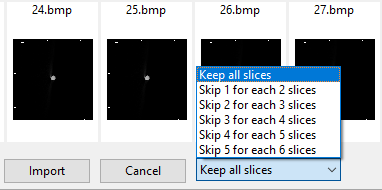
\includegraphics[scale=0.4]{../user_guide_figures/invesalius_screen/import_bmp_skip_en.png}
\caption{Importation window}
\label{fig:import_bmp_skip_pt}
\end{figure}

To reconstruct files of this type, a project name must be defined to indicate the orientation of the images (axial, coronal or sagittal), voxel spacing ($X$, $Y$ and $Z$) in \textbf{mm} as shown in the Figure~\ref{fig:import_bmp_spacing_pt}. The voxel spacing in $X$ is the pixel width of each image, $Y$ the pixel length, and $Z$ represents the distance of each slice (voxel height).

If the image set consists of microtomography images, more specifically GE and Brucker equipment, it is possible that InVesalius will read the text file with the acquisition parameters that normally stay in the same folder as the images and automatically insert the spacing. This verification can be done when the values of $X$, $Y$ and $Z$ are different from "1.00000000", otherwise it is necessary to enter the values of the respective spacing.

\textbf{Correct spacing is crucial for correctly importing objects in InVesalius. Incorrect spacing will provide incorrect measurements.}

Once all parameters have been input, click \textbf{OK}.

\begin{figure}[!htb]
\centering
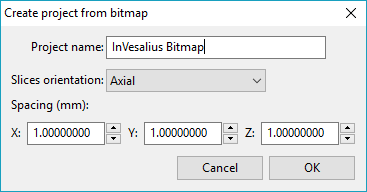
\includegraphics[scale=0.5]{../user_guide_figures/invesalius_screen/import_bmp_spacing_en.png}
\caption{Import Screen}
\label{fig:import_bmp_spacing_pt}
\end{figure}

If insufficient memory is available when loading images, it is recommended to reduce the resolution of the slices to work with volumetric and surface visualization, as shown in Figure~\ref{fig:import_bmp_resize_pt} window.The slices will be resized according to the percentage relative to the original resolution. For example, if each slice of the exam contains the dimension of $512 x 512$ pixels and the "Percentage of the original resolution" is suggested at 60, each resulting image will have $307 x 307$ pixels. If you want to open with the original resolution set the percentage to $100$.

\begin{figure}[!htb]
\centering
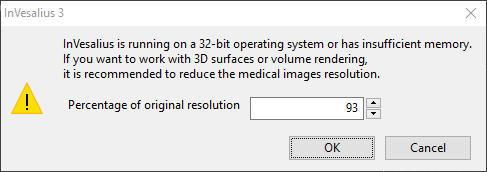
\includegraphics[scale=0.5]{../user_guide_figures/invesalius_screen/import_window_lower_memory_en.png}
\caption{Image resize}
\label{fig:import_bmp_resize_pt}
\end{figure}

After the previous steps, wait a moment for the program to complete the multiplanar reconstruction as shown in Figure~\ref{fig:import_bmp_mpr_pt.png}.

\begin{figure}[!htb]
\centering
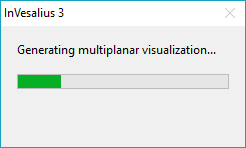
\includegraphics[scale=0.6]{../user_guide_figures/invesalius_screen/import_window_progress_en.png}
\caption{Multiplanar reconstruction in progress.}
\label{fig:import_bmp_mpr_pt.png}
\end{figure}

\chapter{Image adjustment}

InVesalius cannot guarantee the correct image order; images may contain incorrect information, or do not follow the DICOM standard. Therefore, it is recommended to check if a lesion or an anatomical mark is on the correct side. If not, it is possible to use the flip image or swap axes tools. For image alignment, the rotation image tool can be used.

It is possible to mirror the image. To do so, select the \textbf{Tools} menu, click \textbf{Image}, then \textbf{Flip} and click on one of the following options (Figure~\ref{fig:menu_img_mirroring_axis_pt}):

\begin{itemize}
	\item Right - Left
	\item Anterior - Posterior
	\item Top - Botton
\end{itemize}

\begin{figure}[!htb]
\centering
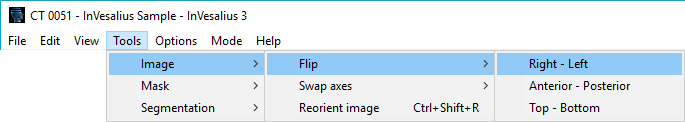
\includegraphics[scale=0.4]{menu_img_mirroring_axis_en.png}
\caption{Menu to activate flip image tool.}
\label{fig:menu_img_mirroring_axis_pt}
\end{figure}


Figure~\ref{fig:mirrored} shows a comparison between the input image and the flipped image. All other orientations are also modified when the image is flipped.

\begin{figure}[!htb]
  \centering
  \subfloat[Input image]{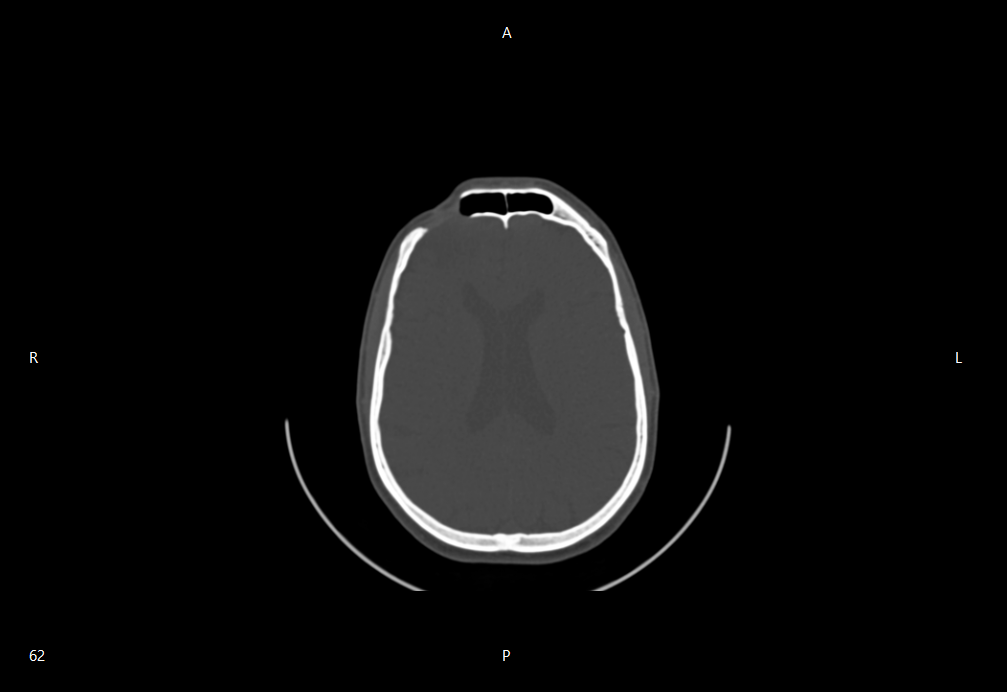
\includegraphics[width=0.45\textwidth]{mirror_axial_en.png}}  \qquad
  \subfloat[Flipped image]{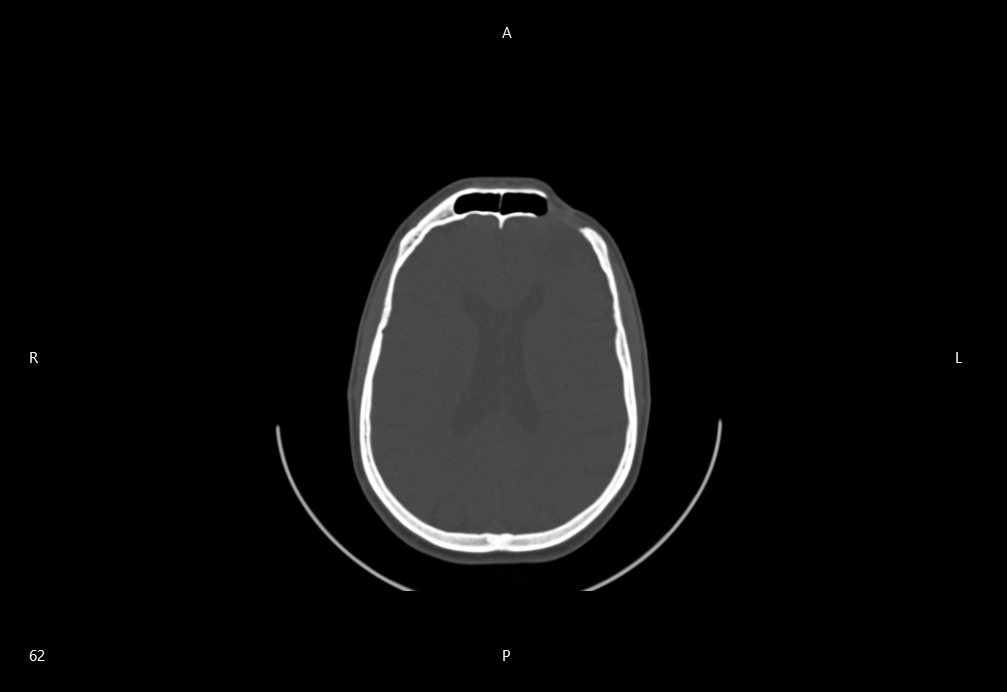
\includegraphics[width=0.45\textwidth]{mirror_axial_mirrored_en.png}}
  \hfill
  \caption{Example of a right-left flipped image.}
  \label{fig:mirrored}
\end{figure}

\section{Swap axes}

The swap axes tool changes the image orientation, in the case that the image has been wrongly imported. To perform this, select the \textbf{Tools} menu, click \textbf{Image}, then \textbf{Swap Axes} and click on one of the following options (Figure~\ref{fig:menu_invert_axis}):

\begin{itemize}
	\item From Right-Left to Anterior-Posterior
	\item From Right-Left to Top-Bottom
	\item From Anterior-Posterior to Top-Bottom
\end{itemize}


The Figures~\ref{fig:invert_axis_axial} and~\ref{fig:invert_axis_axial_inverted}, shows an example of an image with inverted axes.

\begin{figure}[!htb]
\centering
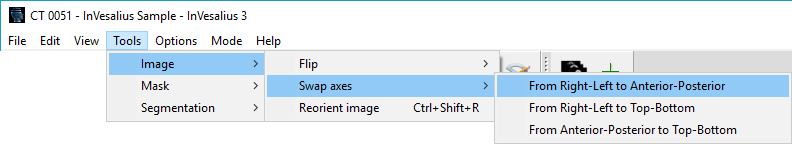
\includegraphics[scale=0.4]{menu_invert_axis_en.png}
\caption{Menu to activate swap image tool.}
\label{fig:menu_invert_axis}
\end{figure}

\begin{figure}[!htb]
\centering
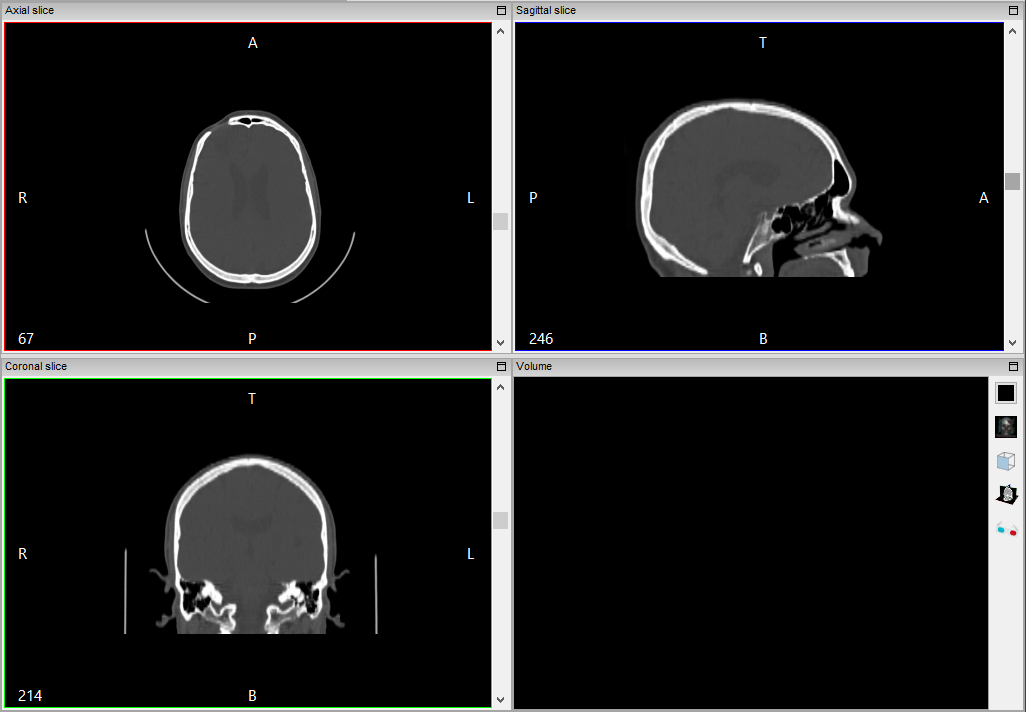
\includegraphics[scale=0.4]{invert_axis_axial_en.png}
\caption{Images before swap axes - from Anterior-Posterior to Top-Bottom.}
\label{fig:invert_axis_axial}
\end{figure}

\begin{figure}[!htb]
\centering
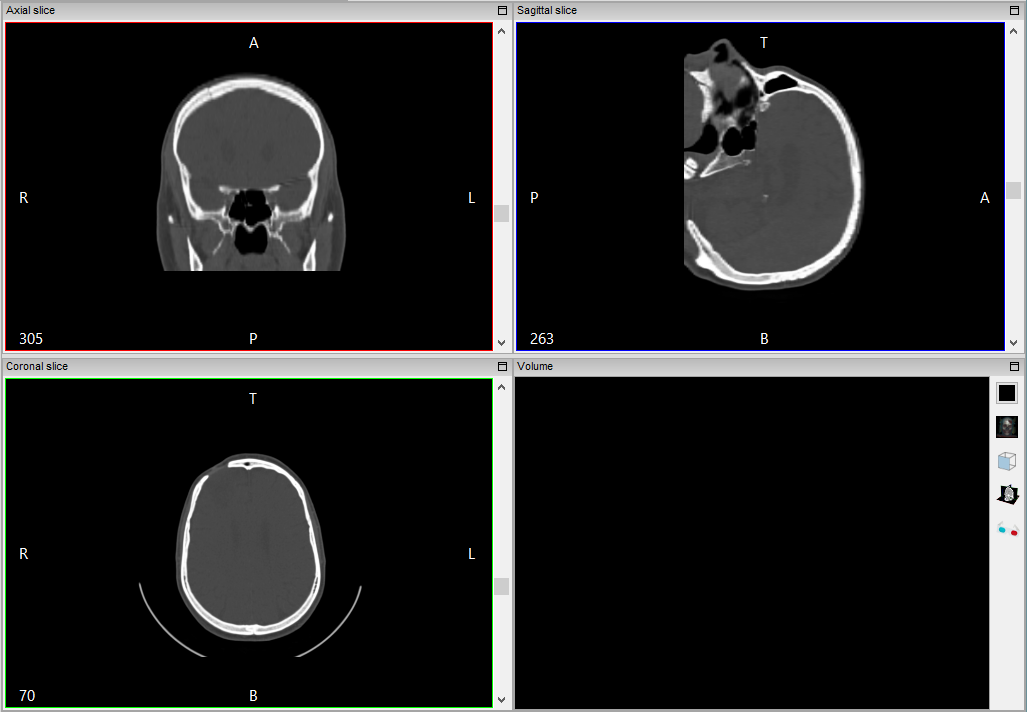
\includegraphics[scale=0.4]{invert_axis_axial_inverted_en.png}
\caption{Images after swap axes - from Anterior-Posterior to Top-Bottom.}
\label{fig:invert_axis_axial_inverted}
\end{figure}

\section{Reorient image (Rotate)}

If it is necessary to align the image with a certain point of reference, e.g. anatomical marker, use the reorient image tool. To open this tool select the \textbf{Tools} menu, click \textbf{Image}, then \textbf{Reorient Image} (Figure~\ref{fig:menu_img_reorient}).

\begin{figure}[!htb]
\centering
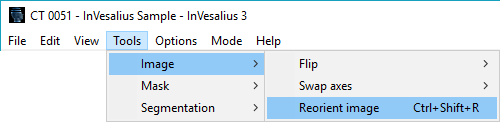
\includegraphics[scale=0.4]{menu_img_reorient_en.png}
\caption{Menu to activate reorient image tool.}
\label{fig:menu_img_reorient}
\end{figure}

When this tool is activated a window is opened (Figure~\ref{fig:image_reorient_window}) showing orientation and by how many degrees the image was rotated.

\begin{figure}[!htb]
\centering
\includegraphics[scale=0.4]{image_reorient_window_en.png}
\caption{Window that shows the reorientation image parameters.}
\label{fig:image_reorient_window}
\end{figure}

To start reorienting the image, define the rotation point by keeping the \textbf{left} mouse button pressed between the two lines intersecting (Figure~\ref{fig:image_reorient_adjust_center}) at one orientation, e.g. axial, coronal or sagittal, and \textbf{drag} to the desired point.

\begin{figure}[!htb]
\centering
\includegraphics[scale=0.4]{image_reorient_adjust_center_en.png}
\caption{Defining the axis of rotation of the image.}
\label{fig:image_reorient_adjust_center}
\end{figure}

To rotate the image it is necessary to keep the \textbf{left} mouse button pressed and \textbf{drag} until the reference point or anatomical marker stays aligned with one of the lines (Figure~\ref{fig:image_reorient_rotated}). After the image is in the desired position, click \textbf{Apply} in the parameter window (Figure~\ref{fig:image_reorient_window}). This may take a few moments depending on the image size. Figure~\ref{fig:image_reorient_rotated_applied} shows an image successfully reoriented.

\begin{figure}[!htb]
\centering
\includegraphics[scale=0.4]{image_reorient_rotated_en.png}
\caption{Rotated image.}
\label{fig:image_reorient_rotated}
\end{figure}

\begin{figure}[!htb]
\centering
\includegraphics[scale=0.4]{image_reorient_rotated_applied_en.png}
\caption{Rotated image after reorientation is done.}
\label{fig:image_reorient_rotated_applied}
\end{figure}

\chapter{Image Manipulation (2D)}

\section{Multiplanar Reconstruction}

When images are imported, InVesalius automatically shows its reconstruction
Multiplanar in the Axial, Sagittal and Coronal orientations, as well as a window for 3D manipulation.
See figure \ref{fig:mpr}.

\begin{figure}[!htb]
\centering
\includegraphics[scale=0.40]{multiplanar_mask_window_en.png}
\caption{Multiplanar Reconstruction}
\label{fig:mpr}
\end{figure}

\newpage

In addition to creating a multiplanar reconstruction, InVesalius segments an image, highlighting, for example, soft tissue bones. The highlight is represented by the application of colors on a segmented structure, i.e., the colors forms a mask over an image highlighting the structure (figure \ref{fig:mpr}). This is discussed in more detail in the following chapters.


To hide the mask, use the data manager, located in the lower left corner
of the screen. Just choose the tab \textbf{Masks} and click \textbf{once} using the
\textbf{left} mouse buttom over the eye icon next to \textbf{"Mask 1"}. See figure
\ref{fig:ger_masc}.

\begin{figure}[!htb]
\centering
\includegraphics[scale=0.8]{data_mask_en.png}
\caption{Mask manager}
\label{fig:ger_masc}
\end{figure}

The eye icon disappears, and the colors of the segmentation mask are hidden (figure
\ref{fig:mpr_sem_mask}).

\begin{figure}[!htb]
\centering
\includegraphics[scale=0.30]{multiplanar_window_en.png}
\caption{Multiplanar reconstruction without segmentation mask}
\label{fig:mpr_sem_mask}
\end{figure}

\subsection{Axial orientation}

The axial orientation consists of cuts made transversal in relation to the region of interest, i.e. parallel cuts to the axial plane of the human body.
In figure \ref{fig:axial_corte}, an axial image of the skull region is displayed.

\begin{figure}[!htb]
\centering
\includegraphics[scale=0.30]{axial_en.png}
\caption{Axial slice}
\label{fig:axial_corte}
\end{figure}

\subsection{Sagittal orientation}

The sagittal orientation consists of cuts made laterally in relation to the region of interest, i.e. parallel cuts to the sagittal plane of the human body, which divides it into the left and right portions.
In figure \ref{fig:sagital_slice}, a sagittal skull image is displayed.

\begin{figure}[!htb]
\centering
\includegraphics[scale=0.30]{sagital_en.png}
\caption{Sagittal slice}
\label{fig:sagital_slice}
\end{figure}

\newpage

\subsection{Coronal orientation}

The coronal orientation is composed of cuts parallel to the coronal plane, which divides the human body into ventral and dorsal halves.
In figure \ref{fig:coronal_slice} is displayed  a skull image in coronal orientation.

\begin{figure}[!htb]
\centering
\includegraphics[scale=0.30]{coronal_en.png}
\caption{Coronal slice}
\label{fig:coronal_slice}
\end{figure}


\section{Correspondence between the axial, sagittal and coronal orientations}
\label{sec:corresp_all_orient}

To find out the common point of the images in differents orientations, simply activate the "Slices cross intersection" feature with the shortcut icon located on the toolbar.
See figure \ref{fig:cross_icon}.

\begin{figure}[!htb]
\centering
\includegraphics[scale=1]{cross.png}
\caption{Shortcut to show common point between different orientations}
\label{fig:cross_icon}
\end{figure}

When the feature is fired, two cross segments that intersect perpendicularly are displayed on each image (figure \ref{fig:cross_all}). The intersection point of each pair of segments represents the common point between differents orientations.

\newpage

To modify the point, keep \textbf{pressed} the \textbf{left} mouse button and
\textbf{drag}. Automatically, the corresponding points will be updated in each image.

\begin{figure}[!htb]
\centering
\includegraphics[scale=0.4]{multiplanar_window_cross_en.png}
\caption{Common point between differents orientations}
\label{fig:cross_all}
\end{figure}

To disable the feature, simply click on the shortcut again (figure \ref{fig:cross_icon}). This feature can be used in conjunction with the slice editor (which will be discussed later).

\section{Interpolation}

By default the 2D images visualization are interpolated (figure~\ref{fig:interp}).a, to deactivate this feature, in menu press \textbf{View}, \textbf{Interpolated slices} (figure~\ref{fig:menu_interpoleted_image_pt}). In this way it will be possible to visualize each pixel individually as shown in the figure~\ref{fig:interp}.b.

\textbf{Note: This interpolation is for visualization purposes only, not directly influencing segmentation or 3D surface generation.}

\begin{figure}[!htb]
\centering
\includegraphics[scale=0.7]{menu_interpoleted_image_en.png}
\caption{Menu to disable and enable interpolation}
\label{fig:menu_interpoleted_image_pt}
\end{figure}


\begin{figure}[!htb]
  \centering
  \subfloat[Interpolated]{\includegraphics[width=0.4\textwidth]{axial_interpoleted.png}}  \qquad
  \subfloat[Non-interpolated]{\includegraphics[width=0.4\textwidth]{axial_not_interpoleted.png}}
  \hfill
  \caption{Interpolated and non-interpolated image visualization.}
  \label{fig:interp}
\end{figure}

\section{Move}

To move an image on the screen, the toolbar's "Move" shortcut icon can be used (figure
\ref{fig:move_icon}). Click on the icon to activate the feature and then with the \textbf{left} mouse button on the image, \textbf{drag} it to the desired direction. The figure \ref{fig:move_img} shows a displaced (moved) image.

\begin{figure}[!htb]
\centering
\includegraphics[scale=0.25]{tool_translate_original.png}
\caption{Shortcut to move images}
\label{fig:move_icon}
\end{figure}

\begin{figure}[!htb]
\centering
\includegraphics[scale=0.20]{axial_pan_en.png}
\caption{Displaced image}
\label{fig:move_img}
\end{figure}

\section{Rotate}

The image rotation can be activated by the toolbar's "Rotate" shortcut icon (figure \ref{fig:rot_icon}). To rotate an image, click on the icon and then with the \textbf{left} mouse button press on the image, \textbf{drag} clockwise or anticlockwise, depending on the desired direction of rotation.

\begin{figure}[!htb]
\centering
\includegraphics[scale=0.20]{tool_rotate_original.png}
\caption{Shortcut to rotate images}
\label{fig:rot_icon}
\end{figure}

\begin{figure}[!htb]
\centering
\includegraphics[scale=0.20]{axial_rotate_en.png}
\caption{Rotated image}
\label{fig:rotate_all}
\end{figure}


\section{Zoom}

In InVesalius, there are different ways to enlarge an image. You can maximize the desired orientation window, apply zoom directly to the image, or select the region of the image to enlarge.

\subsection{Maximizing orientation windows}

As we already know, the main InVesalius window is divided into 4 subwindows: axial, sagittal, coronal and 3D. Each of these can be maximized to occupy the entire area of the main window. To do this, simply \textbf{left} mouse click on the subwindow icon located in the \textbf{upper right corner} (figure \ref{fig:maximize_window}). To restore a maximized window to its previous size, simply click the icon again.

\begin{figure}[!htb]
\centering
\includegraphics[scale=0.6]{maximize_sagital_mpr.png}
\caption{Detail of a sub-window (Note the maximize icon in the upper right corner)}
\label{fig:maximize_window}
\end{figure}

\subsection{Enlarging or reducing an image}

To enlarging or reducing an image, click on the zoom shortcut icon in the toolbar (figure \ref{fig:zoom_icon}). Hold down the \textbf{left} mouse button on the image and \textbf{drag} the mouse to \textbf{top} if you want to enlarge it, or \textbf{down}, if you want to reduce it.

\begin{figure}[!htb]
\centering
\includegraphics[scale=0.25]{tool_zoom_original.png}
\caption{Zoom shortcut}
\label{fig:zoom_icon}
\end{figure}

%\begin{figure}[!htb]
%\centering
%\includegraphics[scale=0.2]{ScreenHunter_76Dec311201_.jpg}
%\caption{Imagem com \textit{Zoom} aplicado}
%\label{fig:zoom_}
%\end{figure}

\subsection{Enlarging an Image Area}

To enlarging a certain image area, click on the "Zoom based on selection" icon in the toolbar (figure \ref{fig:zoom_icon_loc}). Position the mouse pointer at the start position of the selection, click and hold the \textbf{left} mouse button and \textbf{drag} it to the end selection position, forming a rectangle (figure \ref{fig:zoom_select}). Once the left mouse button is released, the zoom operation will be applied to the selected region (figure \ref{fig:zoom_applied}).

\begin{figure}[!htb]
\centering
\includegraphics[scale=0.25]{tool_zoom_select_original.png}
\caption{Zoom based on selection shortcut}
\label{fig:zoom_icon_loc}
\end{figure}

\begin{figure}[!htb]
\centering
\includegraphics[scale=0.25]{tool_zoom_select_image_en.png}
\caption{Area selected for zoom}
\label{fig:zoom_select}
\end{figure}

\begin{figure}[!htb]
\centering
\includegraphics[scale=0.25]{tool_image_with_zoom_en.png}
\caption{Enlarged Image}
\label{fig:zoom_applied}
\end{figure}


\section{Brightness and contrast (Windows)}
\label{sec:ww_wl}

To improve images visualization, the feature \textit{window width} and \textit{window level} can be used, popularly known as "brightness and contrast" or "window" (for radiologists). With this feature, it is possible to set the range of the gray scale (\textit{window level}) and the width of the scale (\textit{window width}) to be used to display the images.

The feature can be triggered by the "Contrast" shortcut icon in the toolbar. See figure \ref{fig:window_level_shortcut}.

\begin{figure}[!htb]
\centering
\includegraphics[scale=0.70]{tool_contrast_original.png}
\caption{Brightness and contrast shortcut}
\label{fig:window_level_shortcut}
\end{figure}

To increase the brightness, hold down the \textbf{left} mouse button and \textbf{drag} horizontally to the right. To decrease the brightness, simply drag the mouse to the left. The contrast can be changed by dragging the mouse (with the \textbf{left} button pressed) vertically: up to increase, or down to decrease the contrast.

To disable the feature, click again on the shortcut icon (figure \ref{fig:window_level_shortcut}).

You can use preset brightness and contrast patterns. The table \ref{tab:window_level} lists some tissues types with their respective brightness and contrast values for the image. To use the presets patterns, position the mouse cursor over the image and \textbf{right-click} to open a context menu on it. When the menu opens, select \textbf{Window width and level}, and then click on the preset option, according to the tissue type, as shown in the figure \ref{fig:window_level}.

\begin{figure}[!htb]
\centering
\includegraphics[scale=0.40]{menu_window_and_level_en.png}
\caption{Context menu for brightness and contrast selection}
\label{fig:window_level}
\end{figure}

\begin{table}[!h]
\centering
\caption{Brightness and contrast values for some tissues}
\begin{tabular}{lcc}\\
\hline % este comando coloca uma linha na tabela
Tissue & Brightness & Contrast\\
\hline
\hline
Default & Exam & Exam\\
Manual & Changed & Changed\\
Abdomen & 350 & 50\\
Bone & 2000 & 300\\
Brain & 80 & 40\\
Brain posterior fossa & 120 & 40\\
Contour & 255 & 127\\
Emphysema & 500 & -850\\
Ischemia - Hard, non contrast & 15 & 32\\
Ischemia - Soft, non contrast & 80 & 20\\
Larynx & 180 & 80\\
Liver & 2000 & -500\\
Lung Hard & 1000 & -600\\
Lung Soft & 1600 & -600\\
Mediastinum & 350 & 25\\
Pelvis & 450 & 50\\
Sinus & 4000 & 400\\
Vasculature - Hard & 240 & 80\\
Vasculature - Soft & 680 & 160\\
\hline
\end{tabular}
\label{tab:window_level}
\end{table} 

\begin{figure}[!h]
  \centering
  \subfloat[Bone]{\label{fig:contrast_bone}\includegraphics[width=0.4\textwidth]{contraste_osso}} \qquad
  \subfloat[Lung]{\label{fig:contrast_isq}\includegraphics[width=0.4\textwidth]{contraste_pulmao}}
  \caption{Different types of brightness and contrast}
  \label{fig:two_window_level}
\end{figure}

\section{Pseudo color}

Another feature to improve the visualization of the images is the pseudo color. They replace gray levels by color, or by inverted gray levels. In the latter case, previously clear regions of the image become darker and vice versa.

To change the view using a pseudo color, position the mouse cursor over the image and \textbf{right-click} to open a context menu on it. When the menu opens, select the entry \textbf{Pseudo color}, and then click on the desired pseudo color option, as shown in the figure \ref{fig:pseudo_color}.

\begin{figure}[p]
\centering
\includegraphics[scale=0.40]{pseudo_menu_en.png}
\caption{Pseudo Color}
\label{fig:pseudo_color}
\end{figure}

Figures \ref{fig:image_default} through \ref{fig:image_saturation} exemplify the various pseudo color options available.

\begin{figure}[h]
  \centering
  \subfloat[Default]{\label{fig:image_default}\includegraphics[width=0.25\textwidth]{pseudo_default.jpg}} \qquad
  \subfloat[Inverted Gray Image]{\label{fig:image_inverted}\includegraphics[width=0.25\textwidth]{pseudo_inverse.jpg}} \qquad
  \subfloat[Rainbow]{\label{fig:image_arc}\includegraphics[width=0.25\textwidth]{pseudo_rainbow.jpg}} \\
  \subfloat[Desert]{\label{fig:image_desert}\includegraphics[width=0.25\textwidth]{pseudo_desert.jpg}} \qquad
  \subfloat[Hue]{\label{fig:image_matiz}\includegraphics[width=0.25\textwidth]{pseudo_hue.jpg}} \qquad
  \subfloat[Ocean]{\label{fig:image_ocean}\includegraphics[width=0.25\textwidth]{pseudo_ocean.jpg}}\\
\subfloat[Saturation]{\label{fig:image_saturation}\includegraphics[width=0.25\textwidth]{pseudo_saturation.jpg}}  
  \caption{Some different types of pseudo-color}
  \label{fig:pseudo_color_types}
\end{figure}

\newpage
\section{Projection type}

It is possible to change the projection type of the 2D images, in addition to the normal mode, InVesalius has six types of projections that can be accessed as follows: Place the mouse over the image and \textbf{rigth-click} to open a context menu on it. When the menu opens, select the projection type option, and then click on the desired projection option, as shown in the figure ~\ref{fig:menu_proj}.

\begin{figure}[!h]
\centering
\includegraphics[scale=0.40]{menu_projection_en.png}
\caption{Projection Type menu}
\label{fig:menu_proj}
\end{figure}

\subsection{Normal}

Normal mode is the default view, i.e. without any type of projection, originally when the image was acquired or customized previously with either brightness and contrast or pseudo color. As shown in figure ~\ref{fig:proj_normal}.

\begin{figure}[!h]
\centering
\includegraphics[scale=0.40]{multiplanar_window_en.png}
\caption{Normal projection}
\label{fig:proj_normal}
\end{figure}

\subsection{MaxIP}
\label{sec:max_ip}
MaxIP is also known as MIP (\textit{Maximum Intensity Projection}), the method selects only voxels that have maximum intensity among the visited ones as shown in figure ~\ref{fig:proj_maxip}. According to the amount or "depth" of MaxIP each voxel is visited in order of overlap, for example, to select MaxIP of the pixel $(0,0)$ consisting of 3 slices it is necessary to visit the pixel $(0,0)$ of slices $(1,2,3)$ and select the highest value.

\begin{figure}[!h]
\centering
\includegraphics[scale=0.40]{multiplanar_window_maxip_en.png}
\caption{MaxIP projection}
\label{fig:proj_maxip}
\end{figure}

As shown in the figure~\ref{fig:proj_maxip_qtd}, the number of images that will be composed of MaxIP is set at the bottom of each orientation image.

\begin{figure}[!h]
\centering
\includegraphics[scale=0.80]{multiplanar_window_maxip_number_en.png}
\caption{Selection the amount of images that composes the MaxIP or MIP}
\label{fig:proj_maxip_qtd}
\end{figure}

\subsection{MinIP}

Unlike MaxIP, MinIP (\textit{Minimun Intensity Projection}) selects only the voxels that have minimal internsity among the visited ones, an example is shown in figure~\ref{fig:proj_minIP}. The image number selection that will compose the projection is made at the bottom of each orientation image as shown in figure~\ref{fig:proj_maxip_qtd}.

\begin{figure}[!h]
\centering
\includegraphics[scale=0.40]{multiplanar_window_minip_en.png}
\caption{MinIP projection}
\label{fig:proj_minIP}
\end{figure}

\subsection{MeanIP}
The MeanIP (\textit{Mean Intensity Projection}) technique which is shown in the figure~\ref{fig:proj_meanIP} composes the projection by averaging the voxels visited. The voxels are visited in the same way as the MaxIP and MinIP methods. It is also possible to define how many images will compose the projection at the bottom of the image of each orientation as shown in the figure~\ref{fig:proj_maxip_qtd}.

\begin{figure}[!h]
\centering
\includegraphics[scale=0.40]{multiplanar_window_mean_en.png}
\caption{MeanIP projection}
\label{fig:proj_meanIP}
\end{figure}

\subsection{MIDA}
\label{sub:mida}
The MIDA (\textit{Maximum Intensity Difference Accumulation}) technique projects an image taking into account only voxels that have local maximum values. From each pixel a ray is simulated towards the volume, each voxel is intercepted by each of these rays reaching the end of the volume, each of these voxels visited has its accumulated value, but are taken into account only if the value is greater than previously visited values. Like MaxIP, you can select how many images are used to accumulate the values. The figure ~\ref{fig:proj_MIDA} shows an example of MIDA projection.

\begin{figure}[!h]
\centering
\includegraphics[scale=0.40]{multiplanar_window_mida_en.png}
\caption{MIDA projection}
\label{fig:proj_MIDA}
\end{figure}

As the figure ~\ref{fig:proj_MIDA_inv} shows, it is possible to invert the order that the voxels are visited by selecting the option \textbf{Inverted order} in the lower corner of the screen.

\begin{figure}[!h]
\centering
\includegraphics[scale=0.40]{multiplanar_window_mida_inverted_en.png}
\caption{Inverted order MIDA projection}
\label{fig:proj_MIDA_inv}
\end{figure}

\subsection{Contour MaxIP}

The technique consists in visualizing contours present in the projection generated with MaxIP technique(\ref{sec:max_ip}). An example is presented in the figure~\ref{fig:proj_contorno_maxip}.

\begin{figure}[!h]
\centering
\includegraphics[scale=0.40]{multiplanar_window_contour_maxip_en.png}
\caption{Contour MaxIP projection}
\label{fig:proj_contorno_maxip}
\end{figure}

\subsection{Contour MIDA}

The technique consists in visualizing contours present in the projection generated with the MIDA technique(\ref{sub:mida}). Like MIDA, you can reverse the order that the volume is visited. We exemplify in the figure~\ref{fig:proj_contorno_mida}.

\begin{figure}[!h]
\centering
\includegraphics[scale=0.40]{multiplanar_window_contour_mida_en.png}
\caption{Contour MIDA projection}
\label{fig:proj_contorno_mida}
\end{figure}
\chapter{Segmentation}

To select a certain type of tissue from an image it is used the segmentation feature at InVesalius.

\section{Threshold}

When using the thresholding segmentation technique, only the pixels whose intensity is inside the threshold range defined by the user are detected. The threshold is defined by two values, the initial (minimum) and final (maximum) threshold.

In thresholding segmentation technique only the \textit{pixels} whose intensity is inside threshold range defined by the user. Threshold is defined by two number, the initial and final threshold, also known as minimum and maximum threshold. ...

Thresholding segmentation is located the InVesalius left-panel, item \textbf{2. Select region of interest} (Figure~\ref{fig:region_selection}).

\begin{figure}[!htb]
\centering
\includegraphics[scale=0.7]{../user_guide_figures/invesalius_screen/segmentation_threshold_window_left_en.png}
\caption{Select region of interest - Threshold}
\label{fig:region_selection}
\end{figure}

Before starting a segment it is necessary to configure a mask. A mask is a image over to examine an image where the selected regions are colored. (Figure~\ref{fig:region_selection_masc}).

\begin{figure}[!htb]
\centering
\includegraphics[scale=0.4]{../user_guide_figures/invesalius_screen/segmentation_threshold_axial_en.png}
\caption{Mask - selected region in yellow.}
\label{fig:region_selection_masc}
\end{figure}

To change the threshold, use the image greyscale control (Figure~\ref{fig:region_selection_bar}). Move the \textit{left} sliding control to change the initial threshold. Move the \textbf{right} sliding control to change the final threshold. It is also possible to to input the desired threshold values in the text boxes in
the left and right side of the thresholding control. The mask will be automatically updated when the thresholding values are changed, showing in color the pixels inside the thresholding range.


\begin{figure}[!htb]
\centering
\includegraphics[scale=0.75]{../user_guide_figures/invesalius_screen/segmentation_threshold_bar.png}
\caption{Selecting \textit{pixels} with intensity between $226$ and $3021$ (Bone)}
\label{fig:region_selection_bar}
\end{figure}

It is also possible to select some predefined thresholding values based on some type of tissues, like those displayed in Figure~\ref{fig:limiar_presets}. Just select the desired tissue and the mask will automatically update.

\begin{figure}[!htb]
\centering
\includegraphics[scale=0.65]{../user_guide_figures/invesalius_screen/segmentation_threshold_presets_en.png}
\caption{Selection list with some predefined thresholding values.}
\label{fig:limiar_presets}
\end{figure}

Table~\ref{tab:limiar} show thresholding values according to some tissues or materials.

\begin{table}[h]
\centering
\caption{Predefined thresholding values to some materials}
\begin{tabular}{lcc}\\
\hline % este comando coloca uma linha na tabela
Material & Initial threshold & Final Threshold\\
\hline
\hline
Bone & 226 & 3021\\
Compact Bone (Adult) & 662 & 1988\\
Compact Bone (Child) & 586 & 2198\\
Custom & User Def. & User Def.\\
Enamel (Adult) & 1553 & 2850\\
Enamel (Child) & 2042 & 3021\\
Fat Tissue (Adult) & -205 & -51\\
Fat Tissue (Child) & -212 & -72\\
Muscle Tissue (Adult) & -5 & 135\\
Muscle Tissue (Child) & -25 & 139\\
Skin Tissue (Adult) & -718 & -177\\
Skin Tissue (Child) & -766 & -202\\
Soft Tissue & -700 & 225\\
Spongial Bone (Adult) & 148 & 661\\
Spongial Bone (Child) & 156 & 585\\
\hline
\end{tabular}
\label{tab:limiar}
\end{table}
\newpage

Table~\ref{tab:limiar} indicates images obtained from medical tomographs. The range of gray values from images obtained from odontological tomographs are greater and non-regular. Thus, it is necessary to use sliding controls (Figure~\ref{fig:region_selection_bar}) to adjust the thresholding values.

To create a new mask, click \textbf{Create new mask} (Figure~\ref{fig:shortcut_new_mask}). Then, click \textbf{Select region of interest}.

\begin{figure}[!htb]
\centering
\includegraphics[scale=0.2]{../user_guide_figures/icons/object_add_original.png}
\caption{Button to create a new mask.}
\label{fig:shortcut_new_mask}
\end{figure}

After clicking on this button a dialog will be shown (Figure~\ref{fig:create_new_mask}). Select the desired threshold and click on \textbf{Ok}.

\begin{figure}[!htb]
\centering
\includegraphics[scale=0.55]{../user_guide_figures/invesalius_screen/segmentation_threshold_window_dialog_en.png}
\caption{Creating a new mask.}
\label{fig:create_new_mask}
\end{figure}

\newpage

After segmentation it is possible to generate a corresponding 3D surface. The surface is formed by triangles. The following chapter will give more details about surfaces.

Click on the \textbf{Create surface} button (Figure~\ref{fig:generate_surface}) to create a new surface. If there is a surface created previously you may overwrite it with the new one. To do this select the option \textbf{Overwrite last surface} before creating the new surface.

\begin{figure}[!htb]
\centering
\includegraphics[scale=0.55]{../user_guide_figures/invesalius_screen/segmentation_generate_surface_en.png}
\caption{Create surface button.}
\label{fig:generate_surface}
\end{figure}

After a few moments the surface will be displayed at the 3D visualization window of InVesalius (Figure~\ref{fig:surface}).

\begin{figure}[!htb]
\centering
\includegraphics[scale=0.5]{../user_guide_figures/invesalius_screen/surface_from_threshold.png}
\caption{3D surface.}
\label{fig:surface}
\end{figure}



\section{Manual segmentation (Image edition)}

Thresholding segmentation may not be efficient in some cases since it is applied to the whole image. Manual segmentation may be used to segment only an isolated region. Manual segmentation also allows users to add or remove some image regions from the segmentation. To use it click on \textbf{Manual edition} (Figure~\ref{fig:advanced_edition}) to open the manual segmentation panel.

\begin{figure}[!htb]
\centering
\includegraphics[scale=0.75]{../user_guide_figures/invesalius_screen/segmentation_manual_label_en.png}
\caption{Icon to open the Manual segmentation panel.}
\label{fig:advanced_edition}
\end{figure}

Figure~\ref{fig:edition_slices_ref} show the Manual segmentation panel.

\begin{figure}[!htb]
\centering
\includegraphics[scale=0.6]{../user_guide_figures/invesalius_screen/segmentation_manual_window_en.png}
\caption{Manual segmentation panel.}
\label{fig:edition_slices_ref}
\end{figure}

There are two brushes used for segmentation: a circle and a square. Click on the triangle icon (see Figure~\ref{fig:brush_type}) to show brush types, then click on the desired brush.

\begin{figure}[!htb]
\centering
\includegraphics[scale=0.9]{../user_guide_figures/invesalius_screen/segmentation_manual_pencil_type.png}
\caption{Brush types.}
\label{fig:brush_type}
\end{figure}

\newpage

Brush sizes can also be adjusted, as shown in Figure~\ref{fig:select_diameter}.

\begin{figure}[!htb]
\centering
\includegraphics[scale=0.8]{../user_guide_figures/invesalius_screen/segmentation_manual_diameter.png}
\caption{Adjusting the brush size.}
\label{fig:select_diameter}
\end{figure}

The following are available options when using brushes in InVesalius:

\begin{itemize}
	\item \textbf{Draw}: for adding a non-selected region to the segmentation;

	\item \textbf{Erase}: for removal of a non-selected region;

	\item \textbf{Threshold}: applies the thresholding locally, adding or removing a region inside or outside of the threshold range.
\end{itemize}

Figure~\ref{fig:select_brush_operations} shows the available brush operations.

\begin{figure}[!htb]
\centering
\includegraphics[scale=0.7]{../user_guide_figures/invesalius_screen/segmentation_manual_pencil_type_operation_type_en.png}
\caption{Brush operations}
\label{fig:select_brush_operations}
\end{figure}

Figure~\ref{fig:noise_amalgaman} shows a image with noise caused by the presence of a dental prosthesis. Note the rays emerging from the dental arch: the thresholding segments the noise since its intensity is inside of the threshold of bone.

\begin{figure}[!htb]
\centering
\includegraphics[scale=0.3]{../user_guide_figures/invesalius_screen/segmentation_manual_noise_amalgam.jpg}
\caption{Noisy image segmented with threshold.}
\label{fig:noise_amalgaman}
\end{figure}

Figure~\ref{fig:surface_amagaman} shows a surface created from that segmentation.

\begin{figure}[!htb]
\centering
\includegraphics[scale=0.3]{../user_guide_figures/invesalius_screen/segmentation_manual_noise_amalgam_3d.jpg}
\caption{Surface generated from noisy image.}
\label{fig:surface_amagaman}
\end{figure}

\begin{figure}[!htb]
\centering
\includegraphics[scale=0.3]{../user_guide_figures/invesalius_screen/segmentation_manual_noise_amalgam_3d_zoom.jpg}
\caption{Zoom in the noisy area.}
\label{fig:surface_amagaman_zoom}
\end{figure}

In such cases use the manual segmentation with the \textbf{erase} brush. Keep the \textbf{left} mouse button pressed while dragging the brush over the region to be removed (in mask).

Figure\ref{fig:editor_amalgaman} shows the image from Figure~\ref{fig:noise_amalgaman} after.

\begin{figure}[!htb]
\centering
\includegraphics[scale=0.3]{../user_guide_figures/invesalius_screen/segmentation_manual_noise_amalgam_removed.jpg}
\caption{After removing the noise.}
\label{fig:editor_amalgaman}
\end{figure}

\begin{figure}[!htb]
\centering
\includegraphics[scale=0.3]{../user_guide_figures/invesalius_screen/segmentation_manual_noise_amalgam_removed_3d_zoom.jpg}
\caption{Surface generate after removing the noise.}
\label{fig:surface_edited_amalgaman}
\end{figure}

A surface can be generated after manual segmentation (Figure~\ref{fig:surface_edited_amalgaman}). Since it was used in the manual segmentation procedure, when clicking on Create surface button, a dialog (Figure~\ref{fig:new_surface_edited}) will be opened to to select if the surface will be created with the method \textbf{Binary} (blocky) or \textbf{Context aware smoothing (smoother)}.

\begin{figure}[!htb]
\centering
\includegraphics[scale=0.5]{../user_guide_figures/invesalius_screen/surface_generation_dialog_en.png}
\caption{Surface creation methods}
\label{fig:new_surface_edited}
\end{figure}


\section{Watershed}

In watershed segmentation the user demarcates objects and background detail. This method treats the image as watershed (hence the name) in which the gray values (intensity) are the altitudes, forming valleys and mountains. The markers are water source. The waters fill the watershed until the waters gather together, thus distinguishing background from object. To use Watershed segmentation click on Watershed to open the watershed panel (Figure~\ref{fig:watershed_painel}).

\begin{figure}[!htb]
\centering
\includegraphics[scale=0.75]{../user_guide_figures/invesalius_screen/segmentation_watershed_panel_en.png}
\caption{Watershed segmentation panel.}
\label{fig:watershed_painel}
\end{figure}

Before segmenting to with Watershed it recommended to clean the mask (see section~\ref{cap:limpeza_mascara}).

To insert a marker (object or background), a brush is used, similar to manual segmenting. You can use a circle or square brush and set its size.

Select brush operations from the following:

\begin{itemize}
    \item \textbf{Object}: to insert object markers;
    \item \textbf{Background}: to insert background markers (not object);
    \item \textbf{Delete}: to delete markers;
\end{itemize}


The option \textbf{Overwrite mask} is used when the user wants the result of watershed segmentation to overwrite the existing segmentation. The option \textbf{Use WWWL} is used to make watershed take into account the image with the values of window width and window level (not the raw image) which may result in better segmentation.

Click on the button on the left side of the panel (Figure~\ref{fig:watershed_conf}) to access more watershed configurations. This button will open a dialog (Figure~\ref{fig:watershed_janela_conf}). The method option allows to choose the Watershed algorithm to be used to segment. It may be the conventional \textbf{Watershed} or \textbf{Watershed IFT}, which is based on the IFT (\textit{Image Forest Transform}) method. In some cases, like brain segmentation, the \textbf{Watershed IFT} may have a better result.

The connectivity option refers to the pixel neighbourhood ($4$ or $8$ when in 2D,  or $6$, $18$ or $26$ when in 3D). \textbf{Gaussian sigma} is a parameter used in the smoothing algorithm (the image is smoothed before the segmentation to remove the noise and get better results). The greater this value the smoother the smoother the image will be.

\begin{figure}[!htb]
    \centering
    \includegraphics[scale=0.5]{../user_guide_figures/icons/configuration.png}
    \caption{Button to open the Watershed configuration dialog.}
    \label{fig:watershed_conf}
\end{figure}

\begin{figure}[!htb]
    \centering
    \includegraphics[scale=0.55]{../user_guide_figures/invesalius_screen/segmentation_watershed_conf_en.png}
    \caption{Watershed configuration dialog.}
    \label{fig:watershed_janela_conf}
\end{figure}

Normally the \textbf{Watershed} is applied only in one slice, not in the whole image. After adding the markers is possible to apply the watershed to the whole image by clicking on the button \textbf{Expand watershed to 3D}. Figure~\ref{fig:watershed_2d} shows the result of watershed segmentation in a slice (2D) of brain image. 

Figure~\ref{fig:watershed_3d} shows the segmentation expanded to the whole image (3D).

Figure~\ref{fig:watershed_2d} also shows the object markers (in light green), the background markers (in red) and the segmentation mask (in green) overlaying the selected regions (result).

\begin{figure}[!htb]
\centering
\includegraphics[scale=0.2]{../user_guide_figures/invesalius_screen/segmentation_watershed_axial.png}
\caption{Watershed applied to a slice.}
\label{fig:watershed_2d}
\end{figure}

\begin{figure}[!htb]
\centering
\includegraphics[scale=0.4]{../user_guide_figures/invesalius_screen/segmentation_watershed_multiplanar_3d_pt.png}
\caption{Brain segmentation using the watershed method applied to the whole image (3D).}
\label{fig:watershed_3d}
\end{figure}

\section{Region growing}

Region growing tool is accessed in the menu \textbf{Tools}, \textbf{Segmentation}, \textbf{Region growing} (figure~\ref{fig:menu_segmentation_region_growing}). Before segmenting select if the operation will be in \textbf{2D - Actual slice} or \textbf{3D - All slices}. It is also necessary to select the connectivity: $4$ or $8$ to 2D or $6$, $18$ or $26$ to 3D. It's also necessary to select the method, which may be \textbf{Dynamic, Threshold, or Confidence} (figure~\ref{fig:segmentation_region_growing_dinamic})

\begin{figure}[!htb]
    \centering
    \includegraphics[scale=0.5]{../user_guide_figures/invesalius_screen/menu_segmentation_region_growing_en.png}
    \caption{Menu to access the region growing segmentation segmentation tool.}
    \label{fig:menu_segmentation_region_growing}
\end{figure}

\begin{figure}[!htb]
    \centering
    \includegraphics[scale=0.7]{../user_guide_figures/invesalius_screen/segmentation_region_growing_dinamic_en.png}
    \caption{Dialog to configure the parameters of region growing segmentation tool.}
    \label{fig:segmentation_region_growing_dinamic}
\end{figure}

This segmentation technique starts with a pixel (indicated by the user left-clicking with the mouse). The selection expands by analyzing the neighbourhood of the selected pixels and including those of a given set of qualities. Each region growing method has a different condition of selection:

\begin{itemize}
	\item \textbf{Dynamic}: Uses the value of the pixel clicked by the user. Then every connected pixel inside the lower (min) and the upper (max) range deviation are selected. The option \textbf{Use WWWL} is default and takes into account the image with \textbf{window width} and \textbf{window level} applied not the raw one (figure~\ref{fig:segmentation_region_growing_dinamic_parameter}).

	\begin{figure}[!htb]
	\centering
	\includegraphics[scale=0.7]{../user_guide_figures/invesalius_screen/segmentation_region_growing_dinamic_parameter_en.png}
	\caption{Dynamic method parameters.}
	\label{fig:segmentation_region_growing_dinamic_parameter}
	\end{figure}

	\item \textbf{Threshold}: This method selects the pixels whose intensity are inside the minimum and maximum threshold (Figure~\ref{fig:segmentation_region_growing_limiar}).

	\begin{figure}[!htb]
	\centering
	\includegraphics[scale=0.7]{../user_guide_figures/invesalius_screen/segmentation_region_growing_limiar_en.png}
    \caption{Adjust the threshold.}
	\label{fig:segmentation_region_growing_limiar}
	\end{figure}

    \item \textbf{Confidence}: This method starts by calculating the standard deviation and the mean value of the pixel selected by the user and its neighbourhood. Connected pixels with value inside the range (given by the mean more and less the standard deviation multiplied by the \textbf{Multiplier} parameter). It then calculates the mean and the standard deviation from the selected pixels, then carries out the expansion.  This process is repeated according to the \textbf{Iterations} parameter. Figure~\ref{fig:segmentation_region_growing_confidence_parameter} shows the parameters for this method.

	\begin{figure}[!htb]
	\centering
	\includegraphics[scale=0.7]{../user_guide_figures/invesalius_screen/segmentation_region_growing_confidence_parameter_en.png}
    \caption{Confidence parameter.}
	\label{fig:segmentation_region_growing_confidence_parameter}
	\end{figure}


\end{itemize}

\chapter{Máscara}


\section{Operações booleanas}

Após efetuar segmentações, é possível realizar operações booleanas entre as máscaras. As operações booleanas suportadas são:

\begin{itemize}
	\item \textbf{União}, realiza a união de duas máscaras;
	\item \textbf{Diferença}, realiza a diferença entre a primeira máscara com a segunda;
	\item \textbf{Intersecção}, para apagar marcadores de objeto ou fundo.
	\item \textbf{Disjunção exclusiva}, também é conhecida como XOR, mantém as regiões de ambas as máscara que possuem diferença.
\end{itemize}

Para ativar essa ferramenta é necessário ir no menu \textbf{Ferramentas}, \textbf{Máscara}, \textbf{Operações boolenas}, como é exibido na figura~\ref{fig:booleano_menu} 

\begin{figure}[!htb]
\centering
\includegraphics[scale=0.5]{../user_guide_figures/invesalius_screen/mask_operation_boolean_menu_pt.png}
\caption{Menu para ativar a ferramenta de operações booleanas.}
\label{fig:booleano_menu}
\end{figure}

É necessário selecionar a primeira máscara, a operação a ser realizada e a segunda máscara conforme mostra a figura~\ref{fig:booleano_janela}. Em seguida é necessário clicar no botão \textbf{Ok}.

\begin{figure}[!htb]
\centering
\includegraphics[scale=0.5]{../user_guide_figures/invesalius_screen/mask_boolean_dialog_pt.png}
\caption{Ferramenta de operações booleanas.}
\label{fig:booleano_janela}
\end{figure}

Na figura~\ref{fig:op_boolana}, apresentamos um exemplo de utilização da ferramenta.

\begin{figure}[!htb]
  \centering
  \subfloat[Máscara A]{\includegraphics[width=0.332\textwidth]{../user_guide_figures/invesalius_screen/booleano_m_a.png}}                
  \hfill
  \subfloat[Máscara B]{\includegraphics[width=0.332\textwidth]{../user_guide_figures/invesalius_screen/booleano_m_b.png}}	
  \hfill  
  \subfloat[União (A $\cup$ B)]{\includegraphics[width=0.332\textwidth]{../user_guide_figures/invesalius_screen/booleano_uniao.png}}
  \hfill  
  \subfloat[Diferença (A - B)]{\includegraphics[width=0.332\textwidth]{../user_guide_figures/invesalius_screen/booleano_dif.png}}
  \hfill  
  \subfloat[Intersecção (A $\cap$ B)]{\includegraphics[width=0.332\textwidth]{../user_guide_figures/invesalius_screen/booleano_interc.png}}
  \hfill  
  \subfloat[Disjunção exclusiva (A $\oplus$ B)]{\includegraphics[width=0.332\textwidth]{../user_guide_figures/invesalius_screen/booleano_disj_exc.png}}
  \caption{Exemplo de operações booleanas.}
  \label{fig:op_boolana}
\end{figure}

\section{Limpeza total da máscara}
\label{cap:limpeza_mascara}

Pode-se efetuar a limpeza total da máscara (figura~\ref{fig:limpeza_mascara}). Isso é recomendado antes de iniciar a inserção de marcadores de Watershed. A ferramenta está localizada no menu \textbf{Ferramentas}, \textbf{Máscara}, \textbf{Limpar máscara}. Também é possível executa-la pressionando as teclas \textbf{CTRL+SHIFT+A}.

\begin{figure}[!htb]
\centering
\includegraphics[scale=0.5]{../user_guide_figures/invesalius_screen/mask_clean_menu_pt.png}
\caption{Limpeza de máscara}
\label{fig:limpeza_mascara}
\end{figure}

\section{Fechar buracos manualmente}

Ao realizar a segmentação é possível que pequenas partes (buracos) que deseja-se ser selecionadas não sejam e ao gerar a superfície para a impressão 3D pode ser que ocorra inconsistências por causa desses buracos, para evitar esse tipo de problema é recomendável preenche-los. Para isso é basta acessar o menu \textbf{Ferramentas}, \textbf{Máscara} e por último clicar em \textbf{Fechar buracos manualmente} (figura~\ref{fig:menu_mask_manual_fill_holes}). Em seguida será exibido uma tela (figura~\ref{fig:mask_manual_fill_holes_window}) para configurar os parâmetros.

\begin{figure}[!htb]
\centering
\includegraphics[scale=0.4]{../user_guide_figures/invesalius_screen/menu_mask_manual_fill_holes_pt.png}
\caption{Menu para acessa a ferramenta de fechamento de buracos manual.}
\label{fig:menu_mask_manual_fill_holes}
\end{figure}

\begin{figure}[!htb]
\centering
\includegraphics[scale=0.7]{../user_guide_figures/invesalius_screen/mask_manual_fill_holes_window_pt.png}
\caption{Tela para configurar parâmetros de fechamento de buracos.}
\label{fig:mask_manual_fill_holes_window}
\end{figure}

Entre os parâmetros existe a opção de realizar o fechamento de buraco levando em consideração somente a fatia atual (\textbf{2D - Fatia Atual}) ou todas as fatias (\textbf{3D - Todas as fatias}) e suas respectivas conectividades, no caso 2D, conectividade $4$ ou $8$, conectividade $6$,$18$ ou $26$. No caso 3D se houver conectividade no buraco em diferentes fatias ele irá expandir para as demais fatias.

Quando os parâmetros estiverem configurados, clique com o \textbf{botão esquerdo} do mouse sobre o buraco que deseja-se fechar.

Podemos observar na imagem~\ref{fig:mask_fill_hole}.a, um exemplo de uma máscara sem preenchimento de buracos e outra com os buracos preenchidos (imagem~\ref{fig:mask_fill_hole}.b). Após o uso da ferramenta, para sair clique no botão \textbf{fechar ou close} no canto inferior direito da janela de configuração de parâmetros.

\begin{figure}[!htb]
  \centering
  \subfloat[Buracos]{\includegraphics[width=0.4\textwidth]{../user_guide_figures/invesalius_screen/mask_axial_with_hole.png}}  \qquad
  \subfloat[Buracos fechados]{\includegraphics[width=0.4\textwidth]{../user_guide_figures/invesalius_screen/mask_axial_filled_hole.png}}
  \hfill
  \caption{Exemplo de máscara com buracos e buracos preenchidos.}
  \label{fig:mask_fill_hole}
\end{figure}


\section{Fechar buracos automaticamente}

Para abrir a ferramenta, no menu do InVesalius clique em \textbf{Ferramentas}, \textbf{Máscara} e por fim \textbf{Fechar buracos automaticamente} (figura~\ref{fig:menu_mask_automatic_fill_holes}), será aberto uma janela para configurar os parâmetros dos buracos que deseja-se fechar. A ferramenta não requer que o usuário clique nos buracos que deseja fechar, ela leva em consideração o tamanho do buraco em voxels que é configurado na janela de configuração de parâmetros (figura~\ref{fig:mask_automatic_fill_holes_window})

\begin{figure}[!htb]
\centering
\includegraphics[scale=0.4]{../user_guide_figures/invesalius_screen/menu_mask_automatic_fill_holes_pt.png}
\caption{Menu para acessar a ferramenta de fechamento de buracos automático.}
\label{fig:menu_mask_automatic_fill_holes}
\end{figure}

\begin{figure}[!htb]
\centering
\includegraphics[scale=0.7]{../user_guide_figures/invesalius_screen/mask_automatic_fill_holes_window_pt.png}
\caption{Tela para configurar parâmetros de fechamento de buracos.}
\label{fig:mask_automatic_fill_holes_window}
\end{figure}

Entre os parâmetros existe a opção de realizar o fechamento de buraco levando em consideração somente a fatia atual (\textbf{2D - Fatia Atual}) ou todas as fatias (\textbf{3D - Todas as fatias}) e suas respectivas conectividades, no caso 2D, conectividade $4$ ou $8$, conectividade $6$,$18$ ou $26$. No caso 2D é necessário indicar qual a janela será aplicado o fechamento de buracos, sendo axial, coronal ou sagital. No caso 3D se houver conectividade no buraco em diferentes fatias ele irá expandir para as demais fatias. 

Com os parâmetros configurados, clique no botão \textbf{Aplicar ou Apply}, caso o resultado não seja satisfatório, reconfigure o tamanho do buraco ou outros parâmetros como conectividade e aplique novamente. Para sair clique no botão \textbf{Sair ou Close}.

\section{Remover partes}

Antes de gerar a superfície é recomendável remover as partes desconexas não desejadas na máscara, dessa forma ao gerar a superfície será utilizada menores quantidades de memória RAM e o processo será mais rápido. Para remover as partes não desejáveis é necessário abrir a ferramenta de remover partes, clicando no menu \textbf{Ferramentas}, \textbf{Máscara} e \textbf{Remover Partes} (figura~\ref{fig:menu_mask_remove_part}). Em seguida irá ser exibido uma janela para configurar os parâmetros de seleção (figura~\ref{fig:mask_remove_parts_window}). É possível selecionar partes desconectas apenas na máscara 2D (\textbf{2D - Fatia atual}) ou em todo o conjunto de imagens, selecionando a opção \textbf{3D - Todas as fatias}. Também é possível selecionar suas respectivas conectividades, no caso 2D, conectividade $4$ ou $8$, conectividade $6$,$18$ ou $26$.

\begin{figure}[!htb]
\centering
\includegraphics[scale=0.4]{../user_guide_figures/invesalius_screen/menu_mask_remove_part_pt.png}
\caption{Menu para acessar a ferramenta de remoção de partes.}
\label{fig:menu_mask_remove_part}
\end{figure}

\begin{figure}[!htb]
\centering
\includegraphics[scale=0.7]{../user_guide_figures/invesalius_screen/mask_remove_parts_window.png}
\caption{Tela para configurar parâmetros de remoção de partes.}
\label{fig:mask_remove_parts_window}
\end{figure}

Selecionado os parâmetros desejados, basta clicar com o \textbf{botão esquerdo do mouse} sobre a região que deseja remover. A figura~\ref{fig:mask_removed_part} apresenta uma exemplo de parte removida e não removida. Para sair da ferramenta clique no botão \textbf{Sair ou Close}.

\begin{figure}[!htb]
  \centering
  \subfloat[Imagem de entrada]{\includegraphics[width=0.45\textwidth]{../user_guide_figures/invesalius_screen/mask_axial_complete.png}}  \qquad
  \subfloat[Imagem com suporte do tomografo removido]{\includegraphics[width=0.45\textwidth]{../user_guide_figures/invesalius_screen/mask_axial_selected_part.png}}
  \hfill
  \caption{Exemplo de região removida na máscara.}
  \label{fig:mask_removed_part}
\end{figure}

\section{Selecionar partes}

Para abrir a ferramenta de seleção de partes desconexas é necessário ir ao menu, \textbf{Ferramentas}, \textbf{Máscara} e por fim \textbf{Selecionar Partes} (figura~\ref{fig:menu_mask_select_part}). A ferramenta irá apresentar uma tela de configuração de parâmetros que consiste em qual conectividade será levada em consideração (figura~\ref{fig:mask_select_part}), podendo ser $6$, $18$ ou $26$ e o nome da nova máscara que irá ter a imagem resultante.

Todas as imagens a região que tem conectividade com o pixel selecionado. Para selecionar o pixel, é necessário clicar com o \textbf{botão esquerdo do mouse} em sobre o pixel desejado, o objeto irá ficar da cor vermelha, é possível selecionar vários objetos. Após a seleção é necessário clicar no \textbf{botão Ok}. A figura~\ref{fig:mask_selected_part}.a apresenta um objeto selecionado na cor vermelha e a figura~\ref{fig:mask_selected_part}.b  somente o objeto após ter fechado a ferramenta (\textbf{botão Ok}).

\begin{figure}[!htb]
\centering
\includegraphics[scale=0.4]{../user_guide_figures/invesalius_screen/menu_mask_select_part_pt.png}
\caption{Menu para acessar a ferramenta de seleção de partes.}
\label{fig:menu_mask_select_part}
\end{figure}

\begin{figure}[!htb]
\centering
\includegraphics[scale=0.7]{../user_guide_figures/invesalius_screen/mask_select_part_pt.png}
\caption{Tela para configurar parâmetros de seleção de partes.}
\label{fig:mask_select_part}
\end{figure}

\begin{figure}[!htb]
  \centering
  \subfloat[Região selecionada em vermelho]{\includegraphics[width=0.45\textwidth]{../user_guide_figures/invesalius_screen/mask_axial_select_part_pt.png}}  \qquad
  \subfloat[Imagem final, somente com a região selecionada]{\includegraphics[width=0.45\textwidth]{../user_guide_figures/invesalius_screen/mask_axial_selected_part_pt.png}}
  \hfill
  \caption{Exemplo de região selecionada na máscara.}
  \label{fig:mask_selected_part}
\end{figure}

\section{Cortar}

É possível cortar parte da máscara afim de selecionar uma região de interesse, isso pode ajudar reduzindo a quantidade de informações a ser processadas ao gerar superfície. Para abrir a ferramenta é necessário ir no menu \textbf{Ferramentas}, \textbf{Máscara} e por último \textbf{Cortar} (figura~\ref{fig:menu_mask_crop}).

\begin{figure}[!htb]
\centering
\includegraphics[scale=0.4]{../user_guide_figures/invesalius_screen/menu_mask_crop_pt.png}
\caption{Menu para acessar a ferramenta de corte.}
\label{fig:menu_mask_crop}
\end{figure}

Será exibida uma caixa delimitadora em cada janela das orientações axial, coronal e sagital.

\chapter{Surface (Triangle mesh)}
\label{cap_surface}

InVesalius, generates 3D surfaces based on image segmentation. A surface is generated using the marching cubes algorithm by transforming voxels from the stacked and segmented images to polygons (triangles in this case).

The controls to configure a 3D surface are accessible on the left panel, under \textbf{3. Configure 3D surface}, \textbf{Surface properties} you have the controls to configure a 3D surface (Figure~\ref{fig:3d_surface_managment}).

\begin{figure}[!htb]
\centering
\includegraphics[scale=0.65]{../user_guide_figures/invesalius_screen/surface_config_panel_en.png}
\caption{3D surface configuration.}
\label{fig:3d_surface_managment}
\end{figure}


\section{Creating 3D surfaces}

News surfaces can be created using an already segmented mask. To do so, on the left panel under \textbf{3. Configure 3D surface}, click on the button shown in Figure~\ref{fig:shortcut_new_surface}.

\begin{figure}[!htb]
\centering
\includegraphics[scale=0.18]{../user_guide_figures/icons/object_add_original.png}
\caption{Button to create a 3D surface.}
\label{fig:shortcut_new_surface}
\end{figure}

After clicking this button a dialog will be shown (Figure~\ref{fig:create_surface_1}). This dialog allows for the configuration of the 3D surface created, including setting the quality of the surface, filling surface holes whilst keeping the largest connected region of the surface intact.

\begin{figure}[!htb]
\centering
\includegraphics[scale=0.5]{../user_guide_figures/invesalius_screen/surface_config_window_en.png}
\caption{3D surface creation dialog.}
\label{fig:create_surface_1}
\end{figure}

The keep largest region option may be used, for instance, to remove the tomograph supports. Figure~\ref{fig:surface_ex1} displays a surface created with \textbf{Keep largest region} and \textbf{Fill holes} activated, whereas Figure~\ref{fig:surface_ex2} displays the surface create without activating that options. Note the tomograph support and the holes.

\begin{figure}[!htb]
  \centering
  \subfloat[Frente]{\label{subfig:surface_ex1_frente}\includegraphics[width=0.338\textwidth]{../user_guide_figures/invesalius_screen/surface_model_front.jpg}}
  \subfloat[Baixo]{\label{subfig:surface_ex1_baixo}\includegraphics[width=0.3\textwidth]{../user_guide_figures/invesalius_screen/surface_model_bottom.jpg}}
  \caption{Surface created with the options \textbf{Keep largest region} and \textbf{Fill holes} activated.}
  \label{fig:surface_ex1}
\end{figure}

\begin{figure}
  \centering
  \subfloat[Frente]{\label{subfig:surface_ex2_frente}\includegraphics[width=0.371\textwidth]{../user_guide_figures/invesalius_screen/surface_model_front_all_parts.jpg}}
  \subfloat[Baixo]{\label{subfig:surface_ex2_baixo}\includegraphics[width=0.3\textwidth]{../user_guide_figures/invesalius_screen/surface_model_bottom_all_parts.jpg}}
  \caption{Surface created with the options \textbf{Keep largest region} and \textbf{Fill holes} deactivated.}
  \label{fig:surface_ex2}
\end{figure}

The \textbf{Surface creation method} item has the following options: \textbf{Binary}, \textbf{Context aware smoothing} and \textbf{Default}. Figure~\ref{fig:surf_method} shows an example of surface created using each of these 3 methods.

The \textbf{Binary} method takes as input the segmentation mask which is binary, where selected regions have value 1 and non-selected have value 0. As it is binary, the surface generated has a blocky aspect, mainly in high curvature areas, appearing staircases.

\textbf{Context aware smoothing} starts generating the surface using Binary, then uses another algorithm in order to smooth the surface to avoid staircase details. This method has 4 parameters presented below.

The \textbf{angle} parameter is the angle between 2 adjacent triangles. If the calculated angle is greater than the angle parameter the triangle will be considered a staircase triangle and will be smoothed. The angle parameter ranges from $0$ to $1$, where $0$ is $0^\circ$ and $1$ is $90^\circ$. The \textbf{Max distance} is the maximum distance that a non-staircase triangle may be from a staircase triangle to be considered to be smoothed. Non-staircase triangles with distance greater than Max distance also will be smoothed but the smoothing will be determined by the \textbf{Min. weight} parameter. This parameter ranges from $0$ (without smoothing) to $1$ (total smoothing). The last parameter, \textbf{N.steps}, is the number of times the smoothing algorithm will be run. The greater this parameter the smoother the surface will be.

The \textbf{Default} method is enabled only when thresholding segmentation was used without any manual modification to the mask. This method does not use the mask image, but the raw image, and generates a smoother surface.

\begin{figure}[!htb]
  \centering
  \subfloat[Binary]{\label{fig:surf_binary}\includegraphics[width=0.33\textwidth]{../user_guide_figures/invesalius_screen/binary.png}}
  \hfill
  \subfloat[Context aware]{\label{fig:surf_context}\includegraphics[width=0.32\textwidth]{../user_guide_figures/invesalius_screen/context.png}}
  \hfill
  \subfloat[Default]{\label{fig:surfa_default}\includegraphics[width=0.332\textwidth]{../user_guide_figures/invesalius_screen/default.png}}
  \caption{Surface generated by each method.}
  \label{fig:surf_method}
\end{figure}

\section{Transparency}

The Transparency function allows for the displaying of a surface transparently. To do so, select the desired surface from the list of surfaces, in the item \textbf{3. Configure 3D surface}, \textbf{Surface properties} (Figure~\ref{fig:select_surface}).

\begin{figure}[!htb]
\centering
\includegraphics[scale=0.8]{../user_guide_figures/invesalius_screen/surface_select_menu_en.png}
\caption{Surface selection.}
\label{fig:select_surface}
\end{figure}

Then, to set the level of surface transparency, use the sliding control shown in Figure~\ref{fig:select_transparency}; the more to the right, the more transparent the surface will be.

\begin{figure}[!htb]
\centering
\includegraphics[scale=0.7]{../user_guide_figures/invesalius_screen/surface_transparency_en.png}
\caption{Selection of surface transparency.}
\label{fig:select_transparency}
\end{figure}

Figure~\ref{fig:model_transparency} shows 2 surfaces: the external surface in green has some level of transparency which permits to see the internal surface in yellow.

\begin{figure}[!htb]
\centering
\includegraphics[scale=0.3]{../user_guide_figures/invesalius_screen/transparency_2.png}
\caption{Surface with transparency.}
\label{fig:model_transparency}
\end{figure}

\newpage

\section{Color}

Surface colors can be altered by selecting the surface (Figure~\ref{fig:select_surface}), and clicking on the colored button on the right of the surface selection list. Figure~\ref{fig:change_surface_color} displays this button, inside item \textbf{3. Configure 3D surface}, \textbf{Surface properties}.

\begin{figure}[!htb]
\centering
\includegraphics[scale=0.6]{../user_guide_figures/invesalius_screen/surface_button_select_color_yellow.png}
\caption{Button to change surface color.}
\label{fig:change_surface_color}
\end{figure}

A dialog will be shown (Figure~\ref{fig:button_select_color}). Select the desired color and click on \textbf{OK}.

\begin{figure}[!htb]
\centering
\includegraphics[scale=0.6]{../user_guide_figures/invesalius_screen/surface_select_color_windows_so_en.png}
\caption{Color dialog.}
\label{fig:button_select_color}
\end{figure}

\section{Splitting disconnected surfaces}

To split disconnected surfaces, select \textbf{3. Configure 3D surface}, \textbf{Advanced options} (Figure~\ref{fig:advanced_tools}).

\begin{figure}[!htb]
\centering
\includegraphics[scale=0.7]{../user_guide_figures/invesalius_screen/surface_painel_advanced_options_en.png}
\caption{Advanced options.}
\label{fig:advanced_tools}
\end{figure}

\newpage

The advanced options panel will be displayed (Figure~\ref{fig:advanced_tools_expanded}).

\begin{figure}[!htb]
\centering
\includegraphics[scale=0.7]{../user_guide_figures/invesalius_screen/surface_split_en.png}
\caption{Advanced options panel.}
\label{fig:advanced_tools_expanded}
\end{figure}

\subsection{Select largest surface}

The option \textbf{Select largest surface} selects, automatically, only surface with the greater volume. Click on the button illustrated in Figure~\ref{fig:short_connectivity_largest}. This operation creates new a surface with only the largest surface.


\begin{figure}[!htb]
\centering
\includegraphics[scale=0.2]{../user_guide_figures/icons/connectivity_largest.png}
\caption{Button to split the largest disconnected surface}
\label{fig:short_connectivity_largest}
\end{figure}

As an example, the Figure~\ref{fig:extract_most_region_1} shows a surface before \textbf{Select largest surface}.

\begin{figure}[!htb]
\centering
\includegraphics[scale=0.3]{../user_guide_figures/invesalius_screen/surface_extract_most_region_1.jpg}
\caption{Disconnected surfaces.}
\label{fig:extract_most_region_1}
\end{figure}

Whereas the Figure~\ref{fig:extract_most_region2} shows the surface with largest disconnected region separated.

\begin{figure}[!htb]
\centering
\includegraphics[scale=0.3]{../user_guide_figures/invesalius_screen/surface_extract_most_region2.jpg}
\caption{Largest disconnected region separated.}
\label{fig:extract_most_region2}
\end{figure}

\newpage

\subsection{Select regions of interest}

Another selection option is Select regions of interest. To do this operation click on the button illustrated in Figure~\ref{fig:short_connectivity_manual}, then click on the desired disconnected surface regions you want to select. Next click on \textbf{Select regions of interest}. This operation will create a new surface with only the selected disconnected regions.

\begin{figure}[!htb]
\centering
\includegraphics[scale=0.2]{../user_guide_figures/icons/connectivity_manual.png}
\caption{Button to select the regions of interest.}
\label{fig:short_connectivity_manual}
\end{figure}

As an example, the Figure~\ref{fig:extract_most_region3} shows the surface created after the user selects the cranium and the right part of the tomograph support.

\begin{figure}[!htb]
\centering
\includegraphics[scale=0.35]{../user_guide_figures/invesalius_screen/surface_extract_most_region3.jpg}
\caption{Example of selected regions of interest}
\label{fig:extract_most_region3}
\end{figure}


\subsection{Split all disconnected surfaces}

Disconnected surface regions can also be split automatically. To do this, click on the button illustrated in Figure\ref{fig:connectivity_split_all}.

\begin{figure}[!htb]
\centering
\includegraphics[scale=0.2]{../user_guide_figures/icons/connectivity_split_all.png}
\caption{Button to split all the disconnected regions surface.}
\label{fig:connectivity_split_all}
\end{figure}

Figure~\ref{fig:extrac_most_region_4} shows an example.

\begin{figure}[!htb]
\centering
\includegraphics[scale=0.3]{../user_guide_figures/invesalius_screen/surface_extract_most_region_4.jpg}
\caption{Example of split all disconnected regions surface.}
\label{fig:extrac_most_region_4}
\end{figure}


\chapter{Medições}

O InVesalius permite realizar medições lineares e angulares em 2D (planos axial,
coronal e sagital) e em 3D (superfícies). Também é possível fazer medições
volumétricas em superfícies.

\section{Medição linear}

Para realizar medições lineares, é necessário ativar o recurso clicando no atalho
correspondente localizado na barra de ferramentas (figura \ref{fig:measure_line_original}).

\begin{figure}[!htb]
\centering
\includegraphics[scale=0.2]{../user_guide_figures/icons/measure_line_original.png}
\caption{Atalho para ativar medição linear}
\label{fig:measure_line_original}
\end{figure}

Uma medição linear é definida entre dois pontos. Com o recurso ativado, clique
\textbf{uma} vez sobre a imagem para estabelecer o ponto inicial. Em seguida,
posicione o ponteiro do mouse no ponto final e clique \textbf{uma} vez novamente.
A medição é executada e o resultado é exibido automaticamente sobre a imagem ou
superfície.

A figura \ref{fig:axial_linear} mostra uma medida linear em 2D na orientação axial,
e a figura \ref{fig:3d_linear} mostra outra medida linear em 3D (superfície).

Uma vez feita a medida linear em 2D, é possível edita-la, para isso é necessário posicionar o mouse sobre uma das extremidades, manter o \textbf{botão direito do mouse} pressionado e arrastar para a posição desejada.

\begin{figure}[!htb]
\centering
\includegraphics[scale=0.4]{../user_guide_figures/invesalius_screen/axial_linear.png}
\caption{Medida linear sobre imagem plana}
\label{fig:axial_linear}
\end{figure}

\begin{figure}[!htb]
\centering
\includegraphics[scale=0.3]{../user_guide_figures/invesalius_screen/3d_linear.jpg}
\caption{Medida linear sobre superfície}
\label{fig:3d_linear}
\end{figure}

\textbf{Nota: A medida linear é dada em milímetros (mm).}

\section{Medição angular}

Uma medição angular em 2D ou sobre uma superfície (3D) pode ser realizada clicando-se
no atalho ilustrado na figura \ref{fig:atalho_angular}.

\begin{figure}[!htb]
\centering
\includegraphics[scale=0.2]{../user_guide_figures/icons/measure_angle_original.jpg}
\caption{Atalho para medição angular}
\label{fig:atalho_angular}
\end{figure}

Para efetuar a medição angular, é necessário fornecer os três pontos que descreverão o
ângulo a ser medido, A\^{B}C. Posicione o ponteiro do mouse e clique \textbf{uma} vez
com o botão esquerdo para determinar o primeiro ponto, A. Para inserir o segundo ponto,
B (o vértice do ângulo ou o "centro do transferidor"), posicione o ponteiro do mouse e
clique \textbf{uma} vez novamente. Repita as mesmas ações para determinar o terceiro
ponto, C. A medição é executada e, automaticamente, a medida resultante é exibida sobre
a imagem ou superfície.

A figura \ref{fig:axial_angular} ilustra uma medida angular em uma imagem plana, e a
figura \ref{fig:axial_superficie} ilustra uma medida angular sobre uma superfície.

A exemplo da medida linear em 2D, também é possível editar a medida angular 2D, para isso é necessário posicionar o mouse sobre uma das extremidades, manter o \textbf{botão direito do mouse} pressionado e arrastar para a posição desejada.

\begin{figure}[!htb]
\centering
\includegraphics[scale=0.38]{../user_guide_figures/invesalius_screen/axial_angular.png}
\caption{Medida angular sobre imagem plana}
\label{fig:axial_angular}
\end{figure}

\begin{figure}[!htb]
\centering
\includegraphics[scale=0.33]{../user_guide_figures/invesalius_screen/angular_superficie.jpg}
\caption{Medida angular sobre superfície}
\label{fig:axial_superficie}
\end{figure}

\textbf{Nota: A medida angular é dada em graus ($^{\circ}$)}


\section{Medição volumétrica}

As medições de volume e área são feitas automaticamente ao se criar uma nova superfície.
Elas são exibidas na aba \textbf{Superfícies 3D}, no painel de gerenciamento de \textbf{Dados}, localizado no canto
inferior esquerdo da tela, como ilustra a figura \ref{fig:volumetric_mensure}.

\begin{figure}[!htb]
\centering
\includegraphics[scale=0.7]{../user_guide_figures/invesalius_screen/painel_volumetric_measures_pt.png}
\caption{Medidas volumétricas}
\label{fig:volumetric_mensure}
\end{figure}

\textbf{Nota: A medida de volume é dada em milímetro cúbico ($mm^3$), já a de área em milímetro quadrado ($mm^2$)}

\chapter{Data management}

We have previously shown how to manipulate surfaces, masks for segmentation and measurements. We can also show or hide, and create or remove these elements in the \textbf{Data} management panel, located in the lower left corner of InVesalius. The panel is divided into 3 tabs: \textbf{Masks}, \textbf{3D Surfaces} and \textbf{Measurements}, as shown in Figure~\ref{fig:volumetric_data}. Each tab contains features corresponding to the elements it refers to.

\begin{figure}[!htb]
\centering
\includegraphics[scale=0.7]{../user_guide_figures/invesalius_screen/painel_mask_manager_en.png}
\caption{Data management}
\label{fig:volumetric_data}
\end{figure}

In each tab, there is a panel divided into rows and columns. The first column of each line determines the visualization status of the listed element. The "eye" icon activates or deactivates the masks, surface or measurement displayed. When one of these elements is being displayed, its corresponding icon (as shown in Figure~\ref{fig:disable_mask}) will also be visible.

\newpage

\begin{figure}[!htb]
\centering
\includegraphics[scale=0.9]{../user_guide_figures/invesalius_screen/eye.jpg}
\caption{Icon indicating the elements visibility}
\label{fig:disable_mask}
\end{figure}

Some operations may be performed with the data. For instance, to remove one element, first select its name, as shown in Figure~\ref{fig:selected_mask}. Next, click in the shortcut shown in Figure~\ref{fig:delete_data}.

\begin{figure}[!htb]
\centering
\includegraphics[scale=0.7]{../user_guide_figures/invesalius_screen/painel_selected_mask_en.png}
\caption{Data selected}
\label{fig:selected_mask}
\end{figure}


\begin{figure}[!htb]
\centering
\includegraphics[scale=0.8]{../user_guide_figures/icons/data_remove.png}
\caption{Remove data}
\label{fig:delete_data}
\end{figure}

To create a new mask, surface or measurement, click on the shortcut shown in Figure~\ref{fig:new_data}, provided that the corresponding tab is open.

\begin{figure}[!htb]
\centering
\includegraphics[scale=0.8]{../user_guide_figures/icons/data_new.png}
\caption{New data}
\label{fig:new_data}
\end{figure}

To duplicate data, select data to be duplicated and click in the shortcut shown in Figure~\ref{fig:duplicate_data}.

\begin{figure}[!htb]
\centering
\includegraphics[scale=0.8]{../user_guide_figures/icons/data_duplicate.png}
\caption{Duplicate data}
\label{fig:duplicate_data}
\end{figure}

\newpage

\section{Masks}

In the Name column, the mask’s color and name are shown. The \textbf{Threshold} column shows the value range used to create the mask. Figure~\ref{fig:volumetric_data} shows an example.

\section{3D Surface}

In the \textbf{Name} column, the surface’s color and name are shown. The \textbf{Volume} column shows the total surface volume. Finally, the \textbf{Transparency} column indicates the level of transparency for use for surface visualization. Figure~\ref{fig:surface_manager} shows an example.

\begin{figure}[!htb]
\centering
\includegraphics[scale=0.7]{../user_guide_figures/invesalius_screen/painel_volumetric_measures_en.png}
\caption{Surface manager}
\label{fig:surface_manager}
\end{figure}

\subsection{Import surface}

We can also import STL, OBJ, PLY or VTP (VTK Polydata File Format) files into an active InVesalius project. To do so, click in the icon shown in Figure~\ref{fig:import_stl}, select the format of the corresponding file, (Figure~\ref{fig:import_surface}) and click Open.

\begin{figure}[!htb]
\centering
\includegraphics[scale=0.8]{../user_guide_figures/icons/load_mesh.png}
\caption{Shortcut to import surface }
\label{fig:import_stl}
\end{figure}

\begin{figure}[!htb]
\centering
\includegraphics[scale=0.4]{../user_guide_figures/invesalius_screen/import_surface_en.png}
\caption{Window to import surface}
\label{fig:import_surface}
\end{figure}

\newpage


\section{Measurements}

The tab Measurements shows the following information. \textbf{Name} indicates the color and measurement name. \textbf{Local} indicates where the measurement was taken (image axial, coronal, sagital or 3D), and \textbf{Type} indicates the type of measurement (linear or angular). Finally, \textbf{Value} shows the measurement value. Figure~\ref{fig:manager_mensuares} illustrates the \textbf{Measurements} tab.

\begin{figure}[!htb]
\centering
\includegraphics[scale=0.7]{../user_guide_figures/invesalius_screen/painel_measures_manager_en.png}
\caption{Data management}
\label{fig:manager_mensuares}
\end{figure}


\chapter{Simultaneous viewing of images and surfaces}

Images and surfaces can be viewed simultaneously by \textbf{left-clicking} on the shortcut (Figure~\ref{fig:slice_plane_original}) located in the lower right corner of the InVesalius interface.

\begin{figure}[!htb]
\centering
\includegraphics[scale=0.6]{slice_plane_original}
\caption{Shortcut for simultaneous viewing}
\label{fig:slice_plane_original}
\end{figure}

This feature allows users to enable or disable the displaying of images in different orientations (or plans) within the same display window of the 3D surface. Simply check or uncheck the corresponding option in the menu shown in Figure~\ref{fig:view_2d_3d_1}.

\begin{figure}[!htb]
\centering
\includegraphics[scale=0.6]{view_2d_3d_1_en.png}
\caption{Selection of the guidelines (plans) to display}
\label{fig:view_2d_3d_1}
\end{figure}

It is worth noting that when a particular orientation is selected, a check is presented in the corresponding option. This is illustrated in Figure~\ref{fig:view_2d_3d_2}.

\begin{figure}[!htb]
\centering
\includegraphics[scale=0.6]{view_2d_3d_2_en.png}
\caption{Selected Guidelines for display}
\label{fig:view_2d_3d_2}
\end{figure}

\newpage

If the surface is already displayed, the plans of the guidelines will be presented as shown in Figure~\ref{fig:only_2d_planes}. Otherwise, only the plans will be displayed.

\begin{figure}[!htb]
\centering
\includegraphics[scale=0.5]{3d_planes}
\caption{Surface and plans displayed simultaneously}
\label{fig:3d_planes}
\end{figure}

\begin{figure}[!htb]
\centering
\includegraphics[scale=0.55]{only_2d_planes}
\caption{Flat display (no surface)}
\label{fig:only_2d_planes}
\end{figure}

\newpage

To view the display of a plan, just uncheck the corresponding option in the menu (Figure~\ref{fig:view_2d_3d_2}).
\chapter{Volume Rendering}
\label{cap:vis_vol}

For volume rendering models, InVesalius employs a technique known as raycasting. Raycasting is a technique that simulates the trace of a beam of light toward the object through each screen pixel. The pixel color is based on the color and transparency of each voxel intercepted by the light beam.

InVesalius contains several pre-defined patterns (presets) to display specific tissue types or different types of exam (tomographic contrast, for example).

To access this feature, simply click the shortcut shown in Figure~\ref{fig:volume_raycasting_origina} in the lower right corner of the screen (next to the surfaces display window) and select one of the available presets.

To turn off volume rendering, click again on the path indicated by Figure~\ref{fig:volume_raycasting_origina} and select the \textbf{Disable} option.

\begin{figure}[!htb]
\centering
\includegraphics[scale=0.4]{volume_raycasting_origina}
\caption{Shortcut to volume visualization}
\label{fig:volume_raycasting_origina}
\end{figure}

\section{Viewing Standards}

There are several predefined viewing patterns. Some examples are illustrated in the following figures.

\begin{figure}[!htb]
\centering
\includegraphics[scale=0.68]{brilhante_I}
\caption{Bright}
\label{fig:brilhante_I}
\end{figure}

\begin{figure}[!htb]
\centering 
\includegraphics[scale=0.65]{vias_aereas_II}
\caption{Airway II}
\label{fig:vias_aereas_II} 
\end{figure}

\begin{figure}[!htb]
\centering
\includegraphics[scale=0.42]{contraste_medio}
\caption{Contrast Medium}
\label{fig:contraste_medio}
\end{figure}

\begin{figure}[!htb]
\centering
\includegraphics[scale=0.55]{MIP}
\caption{MIP}
\label{fig:MIP}
\end{figure}

\newpage

\section{Standard Customization}

Some patterns can be personalized (and customized). Figure~\ref{fig:customize_1} is exhibiting a pattern and some graphical controls adjustment. With these features, the color of a given structure and its opacity can be altered, determining if and how it will be displayed.

\begin{figure}[!htb]
\centering
\includegraphics[scale=0.6]{customize_1}
\caption{Settings for the display pattern Soft Skin + II}
\label{fig:customize_1}
\end{figure}


\newpage

To hide a structure, use the control setting chart to decrease the opacity of the corresponding region. In the example in Figure~\ref{fig:customize_1} suppose we want to hide the muscular part (appearing in red). To do this, simply position the pointer over the muscular part in red and, using the left mouse button, drag the point down to reduce opacity and make the part transparent. Figure~\ref{fig:customize_2} illustrates the result.

Note: The Alpha value indicates the opacity of the color and the \textbf{value}, the color intensity of the pixel.

\begin{figure}[!htb]
\centering
\includegraphics[scale=0.6]{customize_2}
\caption{Display Standard Soft Skin + II changed}
\label{fig:customize_2}
\end{figure}


\newpage

We can also remove or add points on the graph control setting. To remove, simply click with the right mouse button on the point. To add a new point, click the left button on the line graph. One can also save the resulting pattern by clicking the shortcut shown in Figure~\ref{fig:save_preset}.

\begin{figure}[!htb]
\centering
\includegraphics[scale=0.6]{save_preset}
\caption{Shortcut to save standard}
\label{fig:save_preset}
\end{figure}
 
To save the pattern, InVesalius displays a window like the one shown in Figure~\ref{fig:save_window_preset}. Enter a name for the custom pattern and \textbf{click OK}. The saved pattern will be available for the next time the software is opened.

\begin{figure}[!htb]
\centering
\includegraphics[scale=0.7]{save_window_preset_en.png}
\caption{Window to save name of pattern.}
\label{fig:save_window_preset}
\end{figure}

\section{Standard Customization with Brightness and Contrast}

You can customize a pattern without using the graphical control settings presented in the previous section. This is done through the \textbf{brightness and contrast} controls on the toolbar. Activate these by clicking the icon shown in Figure~\ref{fig:tool_contrast_original_vol}.

\begin{figure}[!htb]
\centering
\includegraphics[scale=0.6]{tool_contrast_original}
\caption{Shortcut to Brightness and Contrast}
\label{fig:tool_contrast_original_vol}
\end{figure}

Enable the control by dragging the mouse, with the left button pressed on the volume window. This will change the values of the window width and window level. The procedure is the same as with slices applied to 2D images, which can be seen in section~\ref{sec:ww_wl}. Dragging the mouse in a horizontal direction changes the window level value; drag left to decrease and right to increase. Dragging the mouse vertically changes the value of window width; drag down to decrease and up to increase.

Manipulating these values can be useful for different viewing results. For example, to add tissue to the display, \textbf{drag} the mouse diagonally with \textbf{left button} pressed from the lower right to the upper left corner of the preview window. To remove tissue visualization, do the opposite, (i.e drag the mouse diagonally from top left to bottom right with the left button pressed.). See Figure~\ref{fig:raycasting_add}.

\begin{figure}[!htb]
  \centering
  \subfloat[Bone]{\label{fig:raycasting_add_1}\includegraphics[width=0.33\textwidth]{raycasting_add_1}}                
  \hfill
  \subfloat[Muscle]{\label{fig:raycasting_add_2}\includegraphics[width=0.333\textwidth]{raycasting_add_2}}	
  \hfill  
  \subfloat[Skin]{\label{fig:raycasting_add_3}\includegraphics[width=0.332\textwidth]{raycasting_add_3}}
  \caption{Tissue Addition}
  \label{fig:raycasting_add}
\end{figure}

\newpage

\section{Cut}

In volume rendering, the cut function is used to view a cross-section of a region. With a volume pattern selected, click \textbf{Tools}, and then click \textbf{Cut plane} (Figure~\ref{fig:activate_cut_plane}).

\begin{figure}[!htb]
\centering
\includegraphics[scale=0.4]{activate_cut_plane_en.png}
\caption{Enabling plan to cut}
\label{fig:activate_cut_plane}
\end{figure}

An outline for cutting appears next to the volume. To make the cut, hold the left mouse button on the plane and drag the mouse. To rotate the plane, hold the left mouse button pressed on its edge and move the mouse in the desired direction as shown in Figure~\ref{fig:cutted_image}.

\begin{figure}[!htb]
\centering
\includegraphics[scale=0.6]{cutted_image}
\caption{Image with clipping plane}
\label{fig:cutted_image}
\end{figure}

When finished using the function, click \textbf{Tools} and again click \textbf{Cut plane} (Figure~\ref{fig:cutted_image}).
\chapter{Stereoscopic Visualization}

InVesalius supports stereoscopic visualization of 3D models. First a surface (see chapter~\ref{cap_surface}) or an active volumetric visualization (see chapter~\ref{cap:vis_vol}) must be created. Then, click the icon (shown in Figure~\ref{fig:ster}) on the bottom right part of the interface and choose the desired projection type (Figure~\ref{fig:st_menu}).


\begin{figure}[!htb]
\centering
\includegraphics[scale=0.6]{3D_glasses.png}
\caption{Shortcut to activate stereoscopic viewing methods.}
\label{fig:ster}
\end{figure}

\begin{figure}[!htb]
\centering
\includegraphics[scale=0.4]{st_menu_en.png}
\caption{Different methods of stereoscopic visualization.}
\label{fig:st_menu}
\end{figure}

InVesalius supports the following types of stereoscopic viewing:

\begin{itemize}
	\item Red-blue
	\item Anaglyph
	\item CristalEyes
	\item Interlaced
	\item Left
	\item Right
	\item Dresden
	\item Checkboard
\end{itemize}

Figure~\ref{fig:st_surf_methods} presents three different types of projections.


\begin{figure}[!htb]
  \centering
  \subfloat[Interlaced]{\includegraphics[width=0.3\textwidth]{st_surf_interlaced.jpg}} \qquad
  \subfloat[Anaglyph]{\includegraphics[width=0.3\textwidth]{st_surf_anaglyph.jpg}} \qquad
  \subfloat[Red-blue]{\includegraphics[width=0.3\textwidth]{st_surf_red_blue.jpg}}  
  \hfill
  \caption{Example of different methods of stereoscopic applied on a surface.}
  \label{fig:st_surf_methods}
\end{figure}
\chapter{Exportando dados}

Com o InVesalius, é possível exportar dados para outros softwares, em formatos de arquivo
como OBJ, STL, entre outros.

O menu que contém as opções para exportação localiza-se no painel esquerdo do InVesalius,
dentro do item \textbf{4. Exporte os dados}. Caso o menu não esteja visível, dê um clique
duplo com o botão \textbf{esquerdo} do mouse sobre o item para expandi-lo. A figura
\ref{fig:data_export} mostra esse menu.

\begin{figure}[!htb]
\centering
\includegraphics[scale=0.8]{../user_guide_figures/invesalius_screen/painel_data_export_pt.png}
\caption{Menu para exportação de dados}
\label{fig:data_export}
\end{figure}

\section{Superfície}

Para exportar uma superfície, é necessário selecioná-la no menu de dados, conforme mostra a
figura \ref{fig:data_export_selection}.

\newpage

\begin{figure}[!htb]
\centering
\includegraphics[scale=0.7]{../user_guide_figures/invesalius_screen/painel_data_export_selection_pt.png}
\caption{Seleção de superfície a exportar}
\label{fig:data_export_selection}
\end{figure}

Em seguida, clique sobre o ícone que a figura \ref{fig:surface_export_original} ilustra.

\begin{figure}[!htb]
\centering
\includegraphics[scale=0.2]{../user_guide_figures/icons/surface_export_original.png}
\caption{Atalho para exportar superfície}
\label{fig:surface_export_original}
\end{figure}

Na janela exibida (figura \ref{fig:export_data_window}), insira o nome do arquivo e
selecione o formato desejado para a exportação. Em seguida, clique em \textbf{Salvar}.


\begin{figure}[!htb]
\centering
\includegraphics[scale=0.4]{../user_guide_figures/invesalius_screen/export_surface.png}
\caption{Janela para exportar superfície}
\label{fig:export_data_window}
\end{figure}

Os tipos de arquivo que podem ser exportados estão listados na tabela
\ref{tab:files_export_list}:

\begin{table}[h]
\centering
\caption{Formatos de arquivo que o InVesalius exporta}
\begin{tabular}{lcc}\\
\hline % este comando coloca uma linha na tabela
Formato & Extensão\\
\hline
\hline
Inventor & .iv\\
Polygon File Format & .ply\\
Renderman & .rib\\
Stereolithography (formato binário)& .stl\\
Stereolithography (formato ASCII) & .stl\\
VRML & .vrml\\
VTK PolyData & .vtp\\
Wavefront & .obj\\
\hline
\end{tabular}
\label{tab:files_export_list}
\end{table} 


\section{Imagem}

É possível exportar imagens de qualquer das orientações de exibição (axial, coronal,
sagital e 3D). Para isso, clique com o botão \textbf{esquerdo} do mouse sobre o atalho
exibido na figura \ref{fig:menu_save_image_window} e selecione a sub-janela correspondente
à imagem que deseja exportar.

\begin{figure}[!htb]
\centering
\includegraphics[scale=0.5]{../user_guide_figures/invesalius_screen/menu_save_image_window_pt.png}
\caption{Menu para exportar imagem}
\label{fig:menu_save_image_window}
\end{figure}

Na janela exibida (figura \ref{fig:save_image_window}), selecione o formato do arquivo e
clique no botão \textbf{Salvar}.

\begin{figure}[!htb]
\centering
\includegraphics[scale=0.4]{../user_guide_figures/invesalius_screen/export_bmp_pt.png}
\caption{Janela para exportar imagem}
\label{fig:save_image_window}
\end{figure}

\chapter{Customization}

Some customization options are available for InVesalius users. They are shown as follows.

\section{Tools menu}

To hide/show the side tools menu, click the button shown in Figure~\ref{fig:layout_full_original}.

\begin{figure}[!htb]
\centering
\includegraphics[scale=0.5]{layout_full_original}
\caption{Shortcut to hide/show side tools menu}
\label{fig:layout_full_original}
\end{figure}

With the menu hidden, the image visualization area in InVesalius is expanded, as shown in Figure~\ref{fig:closed_tool_menu}.

\begin{figure}[!htb]
\centering
\includegraphics[scale=0.4]{window_mpr_not_painels_en.png}
\caption{Side menu hidden}
\label{fig:closed_tool_menu}
\end{figure}

\newpage

\section{Automatic positioning of volume/surface}

To automatically set the visualization position of a volume or surface, click on the icon shown in Figure~\ref{fig:3d_automatic_position} (located in the inferior right corner of InVesalius screen) and choose one of the available options for visualization.

\begin{figure}[!htb]
\centering
\includegraphics[scale=0.45]{3d_automatic_position_en.png}
\caption{Options for visualization positioning}
\label{fig:3d_automatic_position}
\end{figure}

\section{Background color of volume/surface window}

To change the background color of the volume/surface window, click on the shortcut shown in Figure~\ref{fig:button_select_color_2}. The shortcut is also located in the lower right corner of the InVesalius screen.

\begin{figure}[!htb]
\centering
\includegraphics[scale=0.8]{colour_button_en.png}
\caption{Shortcut to background color of volume/surface window}
\label{fig:button_select_color_2}
\end{figure}

A window for color selection opens (Figure~\ref{fig:color_window_background}). Next, simply click over the desired color and then click \textbf{OK}.

\begin{figure}[!htb]
\centering
\includegraphics[scale=0.6]{surface_select_color_windows_so_en.png}
\caption{Background color selection}
\label{fig:color_window_background}
\end{figure}

Figure~\ref{fig:background_color} illustrates an InVesalius window with the background color changed.

\begin{figure}[!htb]
\centering
\includegraphics[scale=0.7]{3d_background_changed.png}
\caption{Background color modified}
\label{fig:background_color}
\end{figure}

\newpage

\section{Show/hide text in 2D windows}

To show or hide text in 2D image windows, click on the shortcut illustrated in Figure~\ref{fig:text} on the toolbar.

\begin{figure}[!htb]
\centering
\includegraphics[scale=0.7]{text}
\caption{Shorcut to show or hide texts}
\label{fig:text}
\end{figure}

Figures~\ref{fig:text_on} and~\ref{fig:text_off} show text enabled and disabled, respectively.

\begin{figure}[!htb]
\centering
\includegraphics[scale=0.5]{axial_en.png}
\caption{Show texts enabled}
\label{fig:text_on}
\end{figure}

\begin{figure}[!htb]
\centering
\includegraphics[scale=0.5]{axial_no_tex_en.png}
\caption{Show texts disabled}
\label{fig:text_off}
\end{figure}

\chapter{Neuronavegação}
\label{sec:neuronavegador}

A introdução sobre a neuronavegação é feita na seção~\ref{sec:neuronavegador_intro}, é recomendável a leitura caso não tenha sido feita.

Para utilizar o neuronavegador, é necessário habilitar o modo de neuronavegação do InVesalius selecionando no menu \textbf{Modo} em seguida \textbf{Navegação} (figura~\ref{fig:nav_menu_pt}). Será ativada uma nova aba "Sistema de navegação" que ficará visível no painel à esquerda da janela principal como é apresentado na figura~\ref{fig:nav_painel_pt}.

\begin{figure}[!htb]
\centering
\includegraphics[scale=0.4]{../user_guide_figures/invesalius_screen/nav_menu_pt.png}
\caption{Menu para ativar o modulo de neuronavegação.}
\label{fig:nav_menu_pt}
\end{figure}

\begin{figure}[!htb]
\centering
\includegraphics[scale=0.6]{../user_guide_figures/invesalius_screen/nav_painel_pt.png}
\caption{Aba do sistema de neuronavegação.}
\label{fig:nav_painel_pt}
\end{figure}

\section{Rastreadores espaciais e modo de referência}

O sistema de neuronavegação se comunica com vários sistemas de rastreamento espacial. Atualmente, suporta os dispositivos fabricados pela ClaroNav (figura~\ref{fig:tracker_claron}) e Polhemus (figura~\ref{fig:tracker_polhemus}). 

O usuário deve selecionar o dispositivo correspondente no botão \textbf{Selecione o rastreador:}, figura~\ref{fig:nav_select_tracker}.  Caso o usuário não possua nenhum dos rastreadores suportados e deseja realizar um teste do sistema, deve selecionar a opção \textbf{Depurar rastreador} e realizar normalmente os procedimentos que serão citados a seguir. Nessa opção, trata-se de uma simulação, do qual serão geradas coordenadas aleatórias.

\begin{figure}[!htb]
\centering
\includegraphics[scale=0.4]{../user_guide_figures/tracker_claron.png}
\caption{Rastreador Claron - www.claronav.com/microntracker/.}
\label{fig:tracker_claron}
\end{figure}

\begin{figure}[!htb]
\centering
\includegraphics[scale=0.5]{../user_guide_figures/tracker_polhemus.jpg}
\caption{Rastreador Polhemus - http://polhemus.com/motion-tracking/overview/.}
\label{fig:tracker_polhemus}
\end{figure}

\begin{figure}[!htb]
\centering
\includegraphics[scale=0.5]{../user_guide_figures/invesalius_screen/nav_select_tracker_pt.png}
\caption{Menu para seleção de rastreador.}
\label{fig:nav_select_tracker}
\end{figure}

É possível realizar a navegação com dois diferentes tipos de referência, estático e dinâmico (figura~\ref{fig:nav_menu_ref}). No modo estático as coordenadas do dispositivo de rastreamento são detectadas com apenas uma sonda. Este modo de navegação é chamado de modo de referência estática porque a cabeça dos sujeitos deve permanecer estática na posição em que foram detectados os pontos fiduciais (Mais informações na seção~\ref{sec:corregistro}).
Para evitar problemas relacionados com o movimento da cabeça, alguns dispositivos de rastreamento fornecem uma sonda de referência. A sonda de referência pode ser ligada a uma parte não móvel da cabeça, por exemplo testa, para acompanhar as translações e rotações durante o procedimento de navegação. O uso de uma sonda de referência é o chamado modo de referência dinâmica.

\begin{figure}[!htb]
\centering
\includegraphics[scale=0.5]{../user_guide_figures/invesalius_screen/nav_menu_ref_pt.png}
\caption{Menu para seleção de referência.}
\label{fig:nav_menu_ref}
\end{figure}

\section{Corregistro}
\label{sec:corregistro}

O objetivo do corregistro é estabelecer uma relação entre o espaço de coordenadas do rastreador espacial e o espaço de coordenadas virtual (imagem). Para realizar o corregistro, o usuário deve selecionar três marcadores fiduciais na imagem, para isso primeiramente deverá ativar o recurso de \textbf{Correspondência entre as orientações axial, sagital e coronal} (ver seção~\ref{sec:corresp_all_orient}), coletar as três coordenadas fiduciais usando a sonda do dispositivo de rastreamento. Os fiduciais mais utilizados são o trago auricular esquerdo, trago auricular direito e a fossa nasal. A figura~\ref{fig:nav_selec_coord} ilustra a coleta dos pontos fiduciais. Quando é selecionado algum ponto fiducial na imagem, automaticamente é criado um marcador (esfera da cor verde) no volume, figura~\ref{fig:nav_balls_in_head}.

\begin{figure}[!htb]
\centering
\includegraphics[scale=0.5]{../user_guide_figures/invesalius_screen/nav_selec_coord_pt.png}
\caption{Botões e coordenadas para seleção de pontos fiduciais.}
\label{fig:nav_selec_coord}
\end{figure}

As siglas dos botões para coleta dos fiduciais representam:

\begin{itemize}
	\item OEI: trago auricular esquerdo na imagem
	\item ODI: trago auricular direito na imagem
	\item NAI: fossa nasal na imagem
	\item OER: trago auricular esquerdo no rastreador
	\item OER: trago auricular direito no rastreador
	\item NAR: fossa nasal esquerdo no rastreador
\end{itemize}

\begin{figure}[!htb]
\centering
\includegraphics[scale=0.5]{../user_guide_figures/invesalius_screen/nav_balls_in_head.png}
\caption{Criação de marcadores nos pontos fiduciais da imagem.}
\label{fig:nav_balls_in_head}
\end{figure}


\section{Erro de registro fiducial e navegação}

Após o usuário selecionar os três pontos fiduciais na imagem e os respectivos pontos com o rastreador espacial, o próximo passo é clicar no \textbf{botão Navegar} e o procedimento de navegação será iniciado. Para pausar a navegação, basta clicar novamente no \textbf{botão Navegar}. Automaticamente após selecionado a navegação é calculado o erro de registro fiducial, conhecido como \textit{Fiducial Registration Error} (FRE). Esse erro representa a distância média quadrática do ponto fiducial na imagem com o respectivo ponto fiducial obtido após realizado o corregistro. 

Ao lado do botão de navegação, há a caixa de texto respectivo ao FRE. Se o FRE apresentar um valor alto (acima de 3 mm) a navegação não será precisa e a caixa de texto ficará vermelha, figura~\ref{fig:nav_fre_error}, recomenda-se que o corregistro seja refeito. Caso contrário, para FRE menor que 3 mm a caixa de texto fica verde, representando que a navegação terá precisão aceitável, figura~\ref{fig:nav_fre_ok}.

\begin{figure}[!htb]
\centering
\includegraphics[scale=0.6]{../user_guide_figures/invesalius_screen/nav_fre_error_pt.png}
\caption{Botão de navegação e FRE com valor elevado para navegação.}
\label{fig:nav_fre_error}
\end{figure}

\begin{figure}[!htb]
\centering
\includegraphics[scale=0.6]{../user_guide_figures/invesalius_screen/nav_fre_ok_pt.png}
\caption{Botão de navegação e FRE com valor aceitável para navegação.}
\label{fig:nav_fre_ok}
\end{figure}

\section{Marcadores}

Durante a navegação, é possível criar marcadores esféricos no volume 3D. Para acessar essa função, basta clicar na aba \textbf{Ferramentas extras}, figura~\ref{fig:nav_extra_tools}.

\begin{figure}[!htb]
\centering
\includegraphics[scale=0.6]{../user_guide_figures/invesalius_screen/nav_extra_tools_pt.png}
\caption{Aba para manipulação de marcadores.}
\label{fig:nav_extra_tools}
\end{figure}

A criação de marcadores pode ser executada clicando no botão correspondente, com isso será criado um marcador na posição da cruz vermelha com as características escolhidas na aba, figura~\ref{fig:nav_extra_tools}. O número 4 representa o tamanho do raio da esfera que será criada. Ao lado do tamanho do marcador é possível definir a cor da esfera (figura~\ref{fig:nav_vol_with_markers}). 

Caso o usuário desejar identificar o marcador criado no volume, um \textbf{clique duplo com o botão esquerdo do mouse} deve ser realizado no marcador desejado, com isso o respectivo começará a piscar.

É possível criar uma identificação para o marcador, para isso, deve-se clicar com o botão direto sobre o marcador desejado e selecionar \textbf{Editar ID}, figura~\ref{fig:nav_id_list_markers}, será aberto uma janela para o usuário digitar a identificação, figura~\ref{fig:nav_edit_id_markers}.

\begin{figure}[!htb]
\centering
\includegraphics[scale=0.4]{../user_guide_figures/invesalius_screen/nav_vol_with_markers.png}
\caption{Volume com marcadores em diferentes cores.}
\label{fig:nav_vol_with_markers}
\end{figure} 

\begin{figure}[!htb]
\centering
\includegraphics[scale=0.6]{../user_guide_figures/invesalius_screen/nav_id_list_markers_pt.png}
\caption{Aba para manipulação de marcadores.}
\label{fig:nav_id_list_markers}
\end{figure} 

\begin{figure}[!htb]
\centering
\includegraphics[scale=0.6]{../user_guide_figures/invesalius_screen/nav_edit_id_markers_pt.png}
\caption{Janela para editar identificação do marcador.}
\label{fig:nav_edit_id_markers}
\end{figure} 

A exportação dos marcadores é feita através do \textbf{botão salvar}, a extensão do arquivo gerado é o .mks. Essa extensão de arquivo pode ser aberta por processadores de texto como bloco de notas. O arquivo possui as coordenadas $X$, $Y$ e $Z$ seguido o código $RGB$, tamanho de marcador e a identificação. Posteriormente, esse arquivo pode ser importado através do \textbf{botão Carregar}.

Caso o usuário desejar excluir apenas um marcador basta \textbf{selecionar} o item desejado na lista e clicar no \textbf{botão Remover}, também existe a opção de excluir todos os marcadores criados, \textbf{Deletar todos marcadores}. Além disso, pode-se ocultar/mostrar a exibição dos marcadores no volume pelo \textbf{botão ocultar/mostrar}.

\section{Caixas de seleção, trigger externo}

Outra maneira para criação de marcadores é a monitoração externa de trigger. Para ativa-la basta selecionar a caixa de seleção \textbf{Trigger externo}. Essa função foi desenvolvida para comunicar dispositivos EMT e criar automaticamente o marcador em posições onde os pulsos foram aplicados. No entanto, outras aplicações são possíveis de acordo com a necessidade do usuário.
A comunicação com o dispositivo externo é feita através da porta serial COM1, e basta enviar qualquer sinal do tipo RS-232 em uma velocidade \textit{baud rate} de 9600 no pino de recepção que será criado um marcador na atual posição da cruz.

\section{Câmera do volume}

O posicionamento da câmera do volume é atualizado automaticamente, tanto pela posição da cruz vermelha das fatias quanto pela posição da sonda durante a navegação. O usuário pode desabilitar a atualização automática e atualizar a câmera manualmente. O posicionamento será alterado caso o usuário o fizer na janela de volume.  Para isso, basta desmarcar a caixa de seleção \textbf{Câmera do volume}.

\scalebox{2.0}{\sffamily Autores do Manual}
\\

Paulo Henrique Junqueira Amorim

\href{mailto:paulo.amorim@cti.gov.br}{paulo.amorim@cti.gov.br}
\\


Thiago Franco de Moraes


\href{mailto:thiago.moraes@cti.gov.br}{thiago.moraes@cti.gov.br}
\\

Fábio de Souza Azevedo


\href{mailto:fabio.azevedo@cti.gov.br}{fabio.azevedo@cti.gov.br}
\\


André Salles Cunha Peres (Neuronavegador)

\href{mailto:peres.asc@gmail.com}{peres.asc@gmail.com}
\\

Victor Hugo de Oliveira e Souza  (Neuronavegador)

\href{mailto:victorhos@hotmail.com}{victorhos@hotmail.com}
\\


Renan Hiroshi Matsuda (Neuronavegador)

\href{mailto:renan\_hiroshi@hotmail.com}{renan\_hiroshi@hotmail.com}
\\


Oswaldo Baffa Filho (Neuronavegador)

\href{mailto:baffa@usp.br}{baffa@usp.br}
\\

Jorge Vicente Lopes da Silva


\href{mailto:jorge.silva@cti.gov.br}{jorge.silva@cti.gov.br}
\\


\end{document}


